\section{User guide}

\subsection{Simulator features}

The TMS320C3X is a 32-bit floating-point DSP from Texas Instrument.
The UNISIM TMS320C3X simulator features:
\begin{itemize}
\item Simulation of the TMS320C3X Instruction set
\item A simulation speed average around 10 MIPS and up to 28 MIPS on a 2.4 Ghz Core2 Duo machine under Linux
\item Support for instruction cache
\item Support for TI COFF v0, v1, and v2
\item Built-in debugger (Inline Debugger)
\item Support for GDB serial remote protocol (GDB server)
\item Support for TI C I/O
\end{itemize}

\begin{figure}[!h]
	\begin{center}
		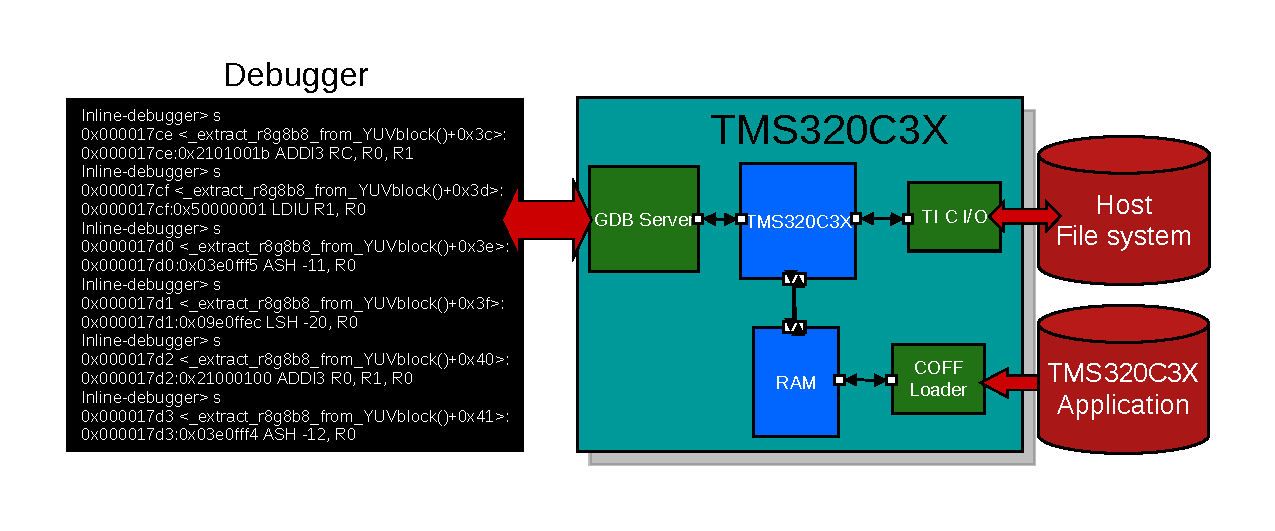
\includegraphics[width=\textwidth]{tms320c3x/fig_tms320c3x.pdf}
	\end{center}
	\caption{TMS320C3X simplified schematic.}
	\label{fig:tms320c3x}
\end{figure}

\subsection{Status of implementation}

The UNISIM TMS320C3X has been developped using the following documentation:
\begin{itemize}
\item TMS320C3x User’s Guide (SPRU031F, 2558539-9761 revision L, March 2004)
\item TMS320C3x/C4x Assembly Language Tools User’s Guide (SPRU035D, June 1998)
\item TMS320C3x/C4x Optimizing C Compiler User’s Guide (SPRU034H, June 1998)
\end{itemize}

Current implementation of the simulator completely decodes the TMS320C3X instruction set.
All registers are present but no on-chip devices are implemented.
The simulator is supposed to have a complete support for:
\begin{itemize}
\item integer instructions (2-ops, 3-ops, parallel ops, load/store)
\item control instructions (branches, delayed branches, RPTS, RPTB)
\item power instructions
\item instructions \texttt{FLOAT}, \texttt{PUSHF}, and \texttt{POPF}
\item interrupt handling
\end{itemize}

The simulator does not implement or partially implement:
\begin{itemize}
\item floating point instructions
\item interlocked instructions
\end{itemize}

The indirect addressing with circular modify and the indirect addressing with bit-reversed modify modes are fully implemented but untested.
The current status of the simulator should allow to run any integer benchmark.

\subsection{Compiling the simulator}

Up-to-date instructions for compiling the simulator are available in file \texttt{INSTALL}.

\subsection{Invoking the simulator}

The general command line format for invoking the simulator is the following:

\begin{verbatim}
tms320c3x [<options>] <binary to simulate>
\end{verbatim}

\noindent The binary to simulate must be a TI's COFF v0, v1 or v2 file. See~\ref{tms320c3x_cross_compiler} to generate such files.
\newline\\
\noindent The command line options of the simulator are:

\begin{itemize}
\item \texttt{--help} or \texttt{-h}: print integrated help message on the screen.
\item \texttt{--get-variables <XML file>} or \texttt{-v <XML file>}: Get the simulation variables (parameters, statistics, \ldots) into a XML file
\item \texttt{--config <XML file>} or \texttt{-c <XML file>}: configures the simulator with the given XML configuration file.
\item \texttt{--get-config <XML file>} or \texttt{-g <XML file>}: Get the simulator default configuration XML file (you can use it to create your own configuration). This option can be combined with option \texttt{-c} to get a new configuration file with existing variables from another file.
\item \texttt{--logger} or \texttt{-l}: Enable the logger.
\item \texttt{--xml-gdb <file>} or \texttt{-x <file>}: processor XML description file for GDB server.
\item \texttt{--gdb-server <port\_number>} or \texttt{-d <port\_number>}: Enable the GDB server and use the given TCP/IP port for communicating with a GDB client.
\item \texttt{--inline-debugger} or \texttt{-i}: Enable the inline debugger (only active if logger option used).
\end{itemize}

\subsection{The Texas Instrument cross-compiler for TMS320C3X}
\label{tms320c3x_cross_compiler}

To compile programs for the TMS320C3X simulator, you can use the free evaluation cross-compiler for TMS320C3X running on a Windows host (SPRC147, TMS320C3x DSK Software) available at \url{http://focus.ti.com/docs/toolsw/folders/print/tmdsdsk33.html}.
This cross-compiler also runs under other x86 operating systems such as Linux or MacOSX using Wine, a Windows emulator (\url{http://www.winehq.org/}).

The cross-compiler tool chain (\texttt{CL30.EXE, LNK30.EXE, ASM30.EXE, MK30.EXE, AR30.EXE, \ldots}) should be in your \texttt{PATH}, for instance:
\begin{verbatim}
set PATH=C:\TI\TIC3X4X\BIN;%PATH%
\end{verbatim}

The shell variable \texttt{C\_DIR} points to the location where cross-compiler should search for the standard C headers and libraries, for instance:
\begin{verbatim}
set C_DIR=C:\TI\TIC3X4X\INCLUDE;C:\TI\TIC3X4X\LIB
\end{verbatim}

Be aware that any call to the C standard library requires linking the program with \texttt{RTS30.LIB}.
Moreover, any call to I/O functions (open, close, read, write, printf, \ldots) requires TI C I/O support enabled in the TMS320C3X simulator.

\subsection{Simulator configuration}
\label{tms320c3x_configuration}

\noindent The simulator stores its configuration (a set of parameters) in a XML configuration file. 
\newline\\
\noindent The simulator can provide the user with a default XML configuration file with option \texttt{-g}:

\begin{verbatim}
$ tms320c3x -g default_sim_config.xml
\end{verbatim}

\noindent The simulator can loads a XML configuration file with option \texttt{-c}:

\begin{verbatim}
$ tms320c3x -c sim_config.xml
\end{verbatim}

\noindent \textit{Note: Although it's not strictly necessary, Parameter \texttt{inline-debugger.memory-atom-size} should be set to value 4 as the TMS320C3X memory is not byte-addressable. If this parameter is not set to 4, presentation of the memory content and disassembly may seem unconventional in the inline debugger.}

\noindent The available parameters are summarized in table below:

\begin{center}
	\tablehead{\hline}
	\tabletail{\hline}
	\begin{supertabular}{|p{7.5cm}|p{7.5cm}|}
	\hline
	\multicolumn{2}{|c|}{\textbf{\large CPU run-time parameters}}\\
	\hline
	\multicolumn{1}{|p{7.5cm}}{\textbf{Name:} \texttt{cpu.max-inst}} & \multicolumn{1}{p{7.5cm}|}{\textbf{Type:} \texttt{64-bit unsigned integer}}\\
	\multicolumn{2}{|p{15cm}|}{\textbf{Default value:} \texttt{$2^{64} - 1$}}\\
	\multicolumn{2}{|l|}{}\\
	\multicolumn{2}{|p{15cm}|}{\textbf{Description:} \newline Maximum number of instructions to execute before stopping simulation.}\\
	\hline
	\multicolumn{1}{|p{7.5cm}}{\textbf{Name:} \texttt{cpu.trap-on-instruction-counter}} & \multicolumn{1}{p{7.5cm}|}{\textbf{Type:} \texttt{64-bit unsigned integer}}\\
	\multicolumn{2}{|p{15cm}|}{\textbf{Default value:} \texttt{$2^{64} - 1$}}\\
	\multicolumn{2}{|l|}{}\\
	\multicolumn{2}{|p{15cm}|}{\textbf{Description:} \newline Number of instructions to execute before leaving control to the debugger.}\\
	\hline
	\multicolumn{1}{|p{7.5cm}}{\textbf{Name:} \texttt{cpu.verbose-all}} & \multicolumn{1}{p{7.5cm}|}{\textbf{Type:} \texttt{bool}}\\
	\multicolumn{2}{|p{15cm}|}{\textbf{Default value:} \texttt{false}}\\
	\multicolumn{2}{|l|}{}\\
	\multicolumn{2}{|p{15cm}|}{\textbf{Description:} \newline Globally enable/disable verbosity of CPU.}\\
	\hline
	\multicolumn{1}{|p{7.5cm}}{\textbf{Name:} \texttt{cpu.verbose-setup}} & \multicolumn{1}{p{7.5cm}|}{\textbf{Type:} \texttt{bool}}\\
	\multicolumn{2}{|p{15cm}|}{\textbf{Default value:} \texttt{false}}\\
	\multicolumn{2}{|l|}{}\\
	\multicolumn{2}{|p{15cm}|}{\textbf{Description:} \newline Enable/disable verbosity of CPU while setup.}\\
	\hline
	\multicolumn{1}{|p{7.5cm}}{\textbf{Name:} \texttt{cpu.verbose-all}} & \multicolumn{1}{p{7.5cm}|}{\textbf{Type:} \texttt{bool}}\\
	\multicolumn{2}{|p{15cm}|}{\textbf{Default value:} \texttt{false}}\\
	\multicolumn{2}{|l|}{}\\
	\multicolumn{2}{|p{15cm}|}{\textbf{Description:} \newline Globally enable/disable verbosity of CPU.}\\
	\hline
	\hline
	\multicolumn{2}{|c|}{\textbf{\large Service GDB Server run-time parameters}}\\
	\hline
	\multicolumn{1}{|p{7.5cm}}{\textbf{Name:} \texttt{gdb-server.tcp-port}} & \multicolumn{1}{p{7.5cm}|}{\textbf{Type:} \texttt{integer}}\\
	\multicolumn{2}{|p{15cm}|}{\textbf{Default value:} \texttt{12345}}\\
	\multicolumn{2}{|l|}{}\\
	\multicolumn{2}{|p{15cm}|}{\textbf{Description:} \newline TCP/IP port to listen waiting for a GDB client connection.}\\
	\hline
	\multicolumn{1}{|p{7.5cm}}{\textbf{Name:} \texttt{gdb-server.architecture-}\newline$\hookrightarrow$\texttt{description-filename}} & \multicolumn{1}{p{7.5cm}|}{\textbf{Type:} \texttt{string}}\\
	\multicolumn{2}{|p{15cm}|}{\textbf{Default value:} \texttt{empty string}}\\
	\multicolumn{2}{|l|}{}\\
	\multicolumn{2}{|p{15cm}|}{\textbf{Description:} \newline Filename of an XML description of the connected processor.}\\
	\hline
	\hline
	\multicolumn{2}{|c|}{\textbf{\large Inline Debugger run-time parameters}}\\
	\hline
	\multicolumn{1}{|p{7.5cm}}{\textbf{Name:} \texttt{inline-debugger.memory-atom-size}} & \multicolumn{1}{p{7.5cm}|}{\textbf{Type:} \texttt{unsigned integer}}\\
	\multicolumn{2}{|p{15cm}|}{\textbf{Default value:} \texttt{1}}\\
	\multicolumn{2}{|l|}{}\\
	\multicolumn{2}{|p{15cm}|}{\textbf{Description:} \newline Size of the smallest addressable element in memory.}\\
	\hline
	\multicolumn{2}{|c|}{\textbf{\large Kernel Service Logger run-time parameters}}\\
	\hline
	\multicolumn{1}{|p{7.5cm}}{\textbf{Name:} \texttt{kernel\_logger.std\_err}} & \multicolumn{1}{p{7.5cm}|}{\textbf{Type:} \texttt{bool}}\\
	\multicolumn{2}{|p{15cm}|}{\textbf{Default value:} \texttt{false}}\\
	\multicolumn{2}{|l|}{}\\
	\multicolumn{2}{|p{15cm}|}{\textbf{Description:} \newline If true, show logger output through the standard error output.}\\
	\hline
	\multicolumn{1}{|p{7.5cm}}{\textbf{Name:} \texttt{kernel\_logger.std\_out}} & \multicolumn{1}{p{7.5cm}|}{\textbf{Type:} \texttt{bool}}\\
	\multicolumn{2}{|p{15cm}|}{\textbf{Default value:} \texttt{false}}\\
	\multicolumn{2}{|l|}{}\\
	\multicolumn{2}{|p{15cm}|}{\textbf{Description:} \newline If true, show logger output through the standard output.}\\
	\hline
	\multicolumn{1}{|p{7.5cm}}{\textbf{Name:} \texttt{kernel\_logger.std\_err\_color}} & \multicolumn{1}{p{7.5cm}|}{\textbf{Type:} \texttt{bool}}\\
	\multicolumn{2}{|p{15cm}|}{\textbf{Default value:} \texttt{false}}\\
	\multicolumn{2}{|l|}{}\\
	\multicolumn{2}{|p{15cm}|}{\textbf{Description:} \newline If true, colorize logger output through the standard error output (only works if std\_err is active).}\\
	\hline
	\multicolumn{1}{|p{7.5cm}}{\textbf{Name:} \texttt{kernel\_logger.std\_out\_color}} & \multicolumn{1}{p{7.5cm}|}{\textbf{Type:} \texttt{bool}}\\
	\multicolumn{2}{|p{15cm}|}{\textbf{Default value:} \texttt{false}}\\
	\multicolumn{2}{|l|}{}\\
	\multicolumn{2}{|p{15cm}|}{\textbf{Description:} \newline If true, colorize logger output through the standard output (only works if std\_out is active).}\\
	\hline
	\multicolumn{1}{|p{7.5cm}}{\textbf{Name:} \texttt{kernel\_logger.file}} & \multicolumn{1}{p{7.5cm}|}{\textbf{Type:} \texttt{bool}}\\
	\multicolumn{2}{|p{15cm}|}{\textbf{Default value:} \texttt{false}}\\
	\multicolumn{2}{|l|}{}\\
	\multicolumn{2}{|p{15cm}|}{\textbf{Description:} \newline If true, keep logger output in a file.}\\
	\hline
	\multicolumn{1}{|p{7.5cm}}{\textbf{Name:} \texttt{kernel\_logger.filename}} & \multicolumn{1}{p{7.5cm}|}{\textbf{Type:} \texttt{string}}\\
	\multicolumn{2}{|p{15cm}|}{\textbf{Default value:} \texttt{empty string}}\\
	\multicolumn{2}{|l|}{}\\
	\multicolumn{2}{|p{15cm}|}{\textbf{Description:} \newline Filename to keep logger output (the option \texttt{file} must be activated).}\\
	\hline
	\multicolumn{1}{|p{7.5cm}}{\textbf{Name:} \texttt{kernel\_logger.xml\_file}} & \multicolumn{1}{p{7.5cm}|}{\textbf{Type:} \texttt{bool}}\\
	\multicolumn{2}{|p{15cm}|}{\textbf{Default value:} \texttt{false}}\\
	\multicolumn{2}{|l|}{}\\
	\multicolumn{2}{|p{15cm}|}{\textbf{Description:} \newline If true, keep logger output in a file XML formatted.}\\
	\hline
	\multicolumn{1}{|p{7.5cm}}{\textbf{Name:} \texttt{kernel\_logger.xml\_filename}} & \multicolumn{1}{p{7.5cm}|}{\textbf{Type:} \texttt{string}}\\
	\multicolumn{2}{|p{15cm}|}{\textbf{Default value:} \texttt{empty string}}\\
	\multicolumn{2}{|l|}{}\\
	\multicolumn{2}{|p{15cm}|}{\textbf{Description:} \newline Filename to keep logger XML output (the option \texttt{xml\_file} must be activated).}\\
	\hline
	\multicolumn{1}{|p{7.5cm}}{\textbf{Name:} \texttt{kernel\_logger.xml\_file\_gzipped}} & \multicolumn{1}{p{7.5cm}|}{\textbf{Type:} \texttt{bool}}\\
	\multicolumn{2}{|p{15cm}|}{\textbf{Default value:} \texttt{false}}\\
	\multicolumn{2}{|l|}{}\\
	\multicolumn{2}{|p{15cm}|}{\textbf{Description:} \newline If the \texttt{xml\_file} option is active, the output file will be compressed (a .gz extension will be automatically added to the \texttt{xml\_filename} option.}\\
	\hline
	\multicolumn{2}{|c|}{\textbf{\large Service COFF Loader run-time parameters}}\\
	\hline
	\multicolumn{1}{|p{7.5cm}}{\textbf{Name:} \texttt{loader.filename}} & \multicolumn{1}{p{7.5cm}|}{\textbf{Type:} \texttt{string}}\\
	\multicolumn{2}{|p{15cm}|}{\textbf{Default value:} \texttt{empty string}}\\
	\multicolumn{2}{|l|}{}\\
	\multicolumn{2}{|p{15cm}|}{\textbf{Description:} \newline The COFF file name to load into memory.}\\
	\hline
	\multicolumn{1}{|p{7.5cm}}{\textbf{Name:} \texttt{loader.dump-headers}} & \multicolumn{1}{p{7.5cm}|}{\textbf{Type:} \texttt{bool}}\\
	\multicolumn{2}{|p{15cm}|}{\textbf{Default value:} \texttt{empty string}}\\
	\multicolumn{2}{|l|}{}\\
	\multicolumn{2}{|p{15cm}|}{\textbf{Description:} \newline If true this parameter makes the COFF loader print the file headers on the screen (file header, section headers, symbol table \ldots) while loading the program.}\\
	\hline
	\multicolumn{2}{|c|}{\textbf{\large Memory run-time parameters}}\\
	\hline
	\multicolumn{1}{|p{7.5cm}}{\textbf{Name:} \texttt{memory.org}} & \multicolumn{1}{p{7.5cm}|}{\textbf{Type:} \texttt{64-bit unsigned integer}}\\
	\multicolumn{2}{|p{15cm}|}{\textbf{Default value:} \texttt{0}}\\
	\multicolumn{2}{|l|}{}\\
	\multicolumn{2}{|p{15cm}|}{\textbf{Description:} \newline Starting address of memory (typically 0).}\\
	\hline
	\multicolumn{1}{|p{7.5cm}}{\textbf{Name:} \texttt{memory.bytesize}} & \multicolumn{1}{p{7.5cm}|}{\textbf{Type:} \texttt{64-bit unsigned integer}}\\
	\multicolumn{2}{|p{15cm}|}{\textbf{Default value:} \texttt{0}}\\
	\multicolumn{2}{|l|}{}\\
	\multicolumn{2}{|p{15cm}|}{\textbf{Description:} \newline Size in bytes (8-bit) of memory.}\\
	\hline
	\hline
	\multicolumn{2}{|c|}{\textbf{\large Service TI C I/O run-time parameters}}\\
	\hline
	\multicolumn{1}{|p{7.5cm}}{\textbf{Name:} \texttt{ti\_c\_io.enable}} & \multicolumn{1}{p{7.5cm}|}{\textbf{Type:} \texttt{bool}}\\
	\multicolumn{2}{|p{15cm}|}{\textbf{Default value:} \texttt{false}}\\
	\multicolumn{2}{|l|}{}\\
	\multicolumn{2}{|p{15cm}|}{\textbf{Description:} \newline Enable/Disable TI C I/O support.}\\
	\hline
	\multicolumn{1}{|p{7.5cm}}{\textbf{Name:} \texttt{ti-c-io.warning-as-error}} & \multicolumn{1}{p{7.5cm}|}{\textbf{Type:} \texttt{bool}}\\
	\multicolumn{2}{|p{15cm}|}{\textbf{Default value:} \texttt{false}}\\
	\multicolumn{2}{|l|}{}\\
	\multicolumn{2}{|p{15cm}|}{\textbf{Description:} \newline Whether Warnings are considered as error or not.}\\
	\hline
	\multicolumn{1}{|p{7.5cm}}{\textbf{Name:} \texttt{ti-c-io.pc-register-name}} & \multicolumn{1}{p{7.5cm}|}{\textbf{Type:} \texttt{string}}\\
	\multicolumn{2}{|p{15cm}|}{\textbf{Default value:} \texttt{"PC"}}\\
	\multicolumn{2}{|l|}{}\\
	\multicolumn{2}{|p{15cm}|}{\textbf{Description:} \newline Name of the CPU program counter register.}\\
	\hline
	\multicolumn{1}{|p{7.5cm}}{\textbf{Name:} \texttt{ti-c-io.c-io-buffer-symbol-name}} & \multicolumn{1}{p{7.5cm}|}{\textbf{Type:} \texttt{string}}\\
	\multicolumn{2}{|p{15cm}|}{\textbf{Default value:} \texttt{"\_\_CIOBUF\_"}}\\
	\multicolumn{2}{|l|}{}\\
	\multicolumn{2}{|p{15cm}|}{\textbf{Description:} \newline C I/O buffer symbol name.}\\
	\hline
	\multicolumn{1}{|p{7.5cm}}{\textbf{Name:} \texttt{ti-c-io.c-io-breakpoint-}\newline$\hookrightarrow$\texttt{symbol-name}} & \multicolumn{1}{p{7.5cm}|}{\textbf{Type:} \texttt{string}}\\
	\multicolumn{2}{|p{15cm}|}{\textbf{Default value:} \texttt{"C\$\$IO\$\$"}}\\
	\multicolumn{2}{|l|}{}\\
	\multicolumn{2}{|p{15cm}|}{\textbf{Description:} \newline C I/O breakpoint symbol name.}\\
	\hline
	\multicolumn{1}{|p{7.5cm}}{\textbf{Name:} \texttt{ti-c-io.c-exit-breakpoint-}\newline$\hookrightarrow$\texttt{symbol-name}} & \multicolumn{1}{p{7.5cm}|}{\textbf{Type:} \texttt{string}}\\
	\multicolumn{2}{|p{15cm}|}{\textbf{Default value:} \texttt{"C\$\$EXIT"}}\\
	\multicolumn{2}{|l|}{}\\
	\multicolumn{2}{|p{15cm}|}{\textbf{Description:} \newline C EXIT breakpoint symbol name.}\\
	\hline
	\multicolumn{1}{|p{7.5cm}}{\textbf{Name:} \texttt{ti-c-io.verbose-all}} & \multicolumn{1}{p{7.5cm}|}{\textbf{Type:} \texttt{bool}}\\
	\multicolumn{2}{|p{15cm}|}{\textbf{Default value:} \texttt{false}}\\
	\multicolumn{2}{|l|}{}\\
	\multicolumn{2}{|p{15cm}|}{\textbf{Description:} \newline Globally enable/disable verbosity of TI C I/O service.}\\
	\hline
	\multicolumn{1}{|p{7.5cm}}{\textbf{Name:} \texttt{ti-c-io.verbose-io}} & \multicolumn{1}{p{7.5cm}|}{\textbf{Type:} \texttt{bool}}\\
	\multicolumn{2}{|p{15cm}|}{\textbf{Default value:} \texttt{false}}\\
	\multicolumn{2}{|l|}{}\\
	\multicolumn{2}{|p{15cm}|}{\textbf{Description:} \newline Enable/disable verbosity of TI C I/O service while I/Os.}\\
	\hline
	\multicolumn{1}{|p{7.5cm}}{\textbf{Name:} \texttt{ti-c-io.verbose-setup}} & \multicolumn{1}{p{7.5cm}|}{\textbf{Type:} \texttt{bool}}\\
	\multicolumn{2}{|p{15cm}|}{\textbf{Default value:} \texttt{false}}\\
	\multicolumn{2}{|l|}{}\\
	\multicolumn{2}{|p{15cm}|}{\textbf{Description:} \newline Enable/disable verbosity of TI C I/O service while setup.}\\
	\hline
	\end{supertabular}
\end{center}

\subsection{Debugging the target program}
\label{tms320c3x_inline_debug}

Command line option \texttt{-i} enables the inline debugger. The inline debugger has support for controling the program execution, inspecting the program and its data, and putting breakpoints and watchpoints. The user can interact with the debugger using the following commands:
\begin{itemize}
\item Execution commands:
	\begin{itemize}
	\item \texttt{<c | cont | continue> [<symbol | *address>]}: \newline
	continue to execute instructions until program reaches a breakpoint, a watchpoint, 'symbol' or 'address'
	\item \texttt{<s | si | step | stepi>}: \newline
	execute one instruction
	\item \texttt{<n | ni | next | nexti>}: \newline
	continue to execute instructions until the processor reaches next contiguous instruction, a breakpoint or a watchpoint
	\item \texttt{<r | run>}: \newline
	restart the simulation from the beginning (not yet supported)
	\end{itemize}
\item Inspection commands:
	\begin{itemize}
	\item \texttt{<dis | disasm | disassemble> [<symbol | *address>]}: \newline
	continue to disassemble starting from 'symbol', 'address', or after the previous disassembly
	\item \texttt{<d | dump> [<symbol | *address>]}: \newline
	dump memory starting from 'symbol', 'address', or after the previous dump
	\item \texttt{<register name>}: \newline
	display the register value
	\item \texttt{<m | monitor> [<variable name>]}: \newline
	display the given simulator variable (displays all variable names if none is given)
	\item \texttt{<p | prof | profile>} \newline
	\texttt{<p | prof | profile> program} \newline
	\texttt{<p | prof | profile> data} \newline
	\texttt{<p | prof | profile> data read} \newline
	\texttt{<p | prof | profile> data write}: \newline
	display the program/data profile
	\end{itemize}
\item Breakpoints/Watchpoints commands:
	\begin{itemize}
	\item \texttt{<b | break> [<symbol | *address>]}: \newline
	set a breakpoint at 'symbol' or 'address'. If 'symbol' or 'address' are not specified, display the breakpoint list
	\item \texttt{<w | watch> [<symbol | *address[:<size>]>] [<read | write>]}: \newline
	set a watchpoint at 'symbol' or 'address'. When using 'continue' and 'next' commands, the debugger will spy CPU loads and store. The debugger will return to command line prompt once a load, or a store will access to 'symbol' or 'address'.
	\item \texttt{<del | delete> <symbol | *address>}: \newline
	delete the breakpoint at 'symbol' or 'address'
	\item \texttt{<delw | delwatch> <symbol | *address> [<read | write>] [<size>]}: \newline
	delete the watchpoint at 'symbol' or 'address'
	\end{itemize}
\item Miscellaneous commands:
	\begin{itemize}
	\item \texttt{<h | ? | help>}: \newline
	display the help
	\item \texttt{<quit | q>}: \newline
	quit the built-in debugger
	\end{itemize}
\end{itemize}

\newpage
\section{Developer guide}

The TMS320C3X simulator is the combination of several software components:
\begin{itemize}
\item A service infrastructure in \texttt{unisim/kernel/service} (see ~\ref{tms320c3x_service_infrastructure})
\item A built-in logger in \texttt{unisim/kernel/logger} (see ~\ref{tms320c3x_logger})
\item Several small utility classes in \texttt{unisim/util} (see ~\ref{tms320c3x_utils})
\item A TMS320C3X instruction set simulator in \texttt{unisim/component/cxx/processor/tms320} (see ~\ref{tms320c3x_iss})
\item A memory in \texttt{unisim/component/cxx/memory/ram} (see ~\ref{tms320c3x_memory})
\item Service interface definitions in \texttt{unisim/service/interfaces} (see ~\ref{tms320c3x_interfaces})
\item A COFF loader service in \texttt{unisim/service/loader/coff\_loader} (see ~\ref{tms320c3x_coff_loader})
\item A TI C I/O service in \texttt{unisim/service/os/ti\_c\_io} (see ~\ref{tms320c3x_ti_c_io})
\item An inline debugger service in \texttt{unisim/service/debug/inline\_debugger} (see ~\ref{tms320c3x_inline_debugger})
\item A GDB server service in \texttt{unisim/service/debug/gdb\_server} (see ~\ref{tms320c3x_gdb_server})
\end{itemize}

\subsection{Simulation Components}

\subsubsection{TMS320C3X instruction set simulator}
\label{tms320c3x_iss}

The instruction set simulator source code is located in directory: \newline \texttt{unisim/component/cxx/processor/tms320}.\newline
The UNISIM TMS320C3X instruction set simulator uses an instruction set simulator generator, GenISSLib.
GenISSLib uses an instruction set description (\texttt{.isa} files) located in sub-directory \texttt{isa} of the instruction set simulator source code directory.
Most computations (e.g. integer computation) are directly performed in these description file.
See the GenISSLib manual for additional informations about the GenISSLib instruction set description language.
The simulator is implemented in class \texttt{unisim::component::cxx::processor::tms320::CPU} which main methods are:
\begin{itemize}
\item \texttt{StepInstruction}: executes one instruction
\item \texttt{PrWrite}: Write a word into memory using service import \texttt{memory\_import}. This methods is virtual so that it can be reimplemented into a derived class.
\item \texttt{PrRead}: Read a word from memory using service import \texttt{memory\_import}. This methods is virtual so that it can be reimplemented into a derived class.
\item \texttt{SetIRQLevel}: Set level (0/1, true/false) of an IRQ. IRQ numbering is same as register \texttt{IF} bit numbering.
\item \texttt{ComputeIndirEA}: Compute the effective address for indirect addressing modes.
\item \texttt{ComputeDirEA}: Compute the effective address for direct addressing modes.
\end{itemize}

Each register (R0, R1, R2, R3, R4, R5, R6, R7, AR0, AR1, AR2, AR3, AR4, AR5, AR6, AR7, DP, IR0, IR1, BK, SP, ST, IE, IF, IOF, RS, RE, and RC) is implemented by an instance of class \texttt{unisim::component::cxx::processor::tms320::Register}.
This class has methods to get/set value of a register and to perform floating point computations.

\noindent The table below summarizes the API of the CPU:

\begin{center}
	\tablehead{\hline}
	\tabletail{\hline}
	\begin{supertabular}{|p{7.5cm}|p{7.5cm}|}
		\hline
		\multicolumn{2}{|l|}{\textbf{\Large Module CPU}}\\
		\hline
		\multicolumn{1}{|p{7.5cm}}{\textbf{Class Name:} \newline \texttt{unisim::component::cxx::processor}\newline$\hookrightarrow$\texttt{::tms320::CPU}} & \multicolumn{1}{p{7.5cm}|}{\textbf{Header:} \newline \texttt{unisim/component/cxx/processor}\newline$\hookrightarrow$\texttt{/tms320/cpu.hh}}\\
		\multicolumn{2}{|l|}{}\\
		\multicolumn{2}{|p{15cm}|}{\textbf{Description:} \newline This C++ class is TMS320C3X instruction set simulator.}\\
		\hline
		\hline
		\multicolumn{2}{|c|}{\textbf{\large Template Parameters}}\\
		\hline
		\multicolumn{1}{|p{7.5cm}}{\textbf{Name:} \texttt{CONFIG}} & \multicolumn{1}{p{7.5cm}|}{\textbf{Type:} \texttt{class}}\\
		\multicolumn{2}{|p{15cm}|}{\textbf{Default value:} \texttt{none}}\\
		\multicolumn{2}{|l|}{}\\
		\multicolumn{2}{|p{15cm}|}{\textbf{Description:} \newline This is a configuration class that is a collection of definitions to parameterize the simulation model.}\\
		\hline
		\multicolumn{1}{|p{7.5cm}}{\textbf{Name:} \texttt{DEBUG}} & \multicolumn{1}{p{7.5cm}|}{\textbf{Type:} \texttt{bool}}\\
		\multicolumn{2}{|p{15cm}|}{\textbf{Default value:} \texttt{false}}\\
		\multicolumn{2}{|l|}{}\\
		\multicolumn{2}{|p{15cm}|}{\textbf{Description:} \newline Enable/Disable debug.}\\
		\hline
		\hline
		\multicolumn{2}{|c|}{\textbf{\large Run-Time Parameters}}\\
		\hline
		\multicolumn{1}{|p{7.5cm}}{\textbf{Name:} \texttt{max-inst}} & \multicolumn{1}{p{7.5cm}|}{\textbf{Type:} \texttt{uint64\_t}}\\
		\multicolumn{2}{|p{15cm}|}{\textbf{Default value:} \texttt{$2^{64} - 1$}}\\
		\multicolumn{2}{|l|}{}\\
		\multicolumn{2}{|p{15cm}|}{\textbf{Description:} \newline Maximum number of instructions to simulate. Once this threshold is reached, the CPU calls virtual method \texttt{Stop} to stop simulation.}\\
		\hline
		\multicolumn{1}{|p{7.5cm}}{\textbf{Name:} \texttt{trap-on-instruction-counter}} & \multicolumn{1}{p{7.5cm}|}{\textbf{Type:} \texttt{uint64\_t}}\\
		\multicolumn{2}{|p{15cm}|}{\textbf{Default value:} \texttt{$2^{64} - 1$}}\\
		\multicolumn{2}{|l|}{}\\
		\multicolumn{2}{|p{15cm}|}{\textbf{Description:} \newline Number of instructions to simulate before traping, i.e. calling \texttt{ReportTrap} through service import \texttt{trap\_import}. This is useful to inform debugger that CPU has simulated a certain amount of instructions, so that user can take control of the simulation at this point.}\\
		\hline
		\multicolumn{1}{|p{7.5cm}}{\textbf{Name:} \texttt{verbose-setup}} & \multicolumn{1}{p{7.5cm}|}{\textbf{Type:} \texttt{bool}}\\
		\multicolumn{2}{|p{15cm}|}{\textbf{Default value:} \texttt{false}}\\
		\multicolumn{2}{|l|}{}\\
		\multicolumn{2}{|p{15cm}|}{\textbf{Description:} \newline Enable/disable verbosity of CPU while setup.}\\
		\hline
		\multicolumn{1}{|p{7.5cm}}{\textbf{Name:} \texttt{verbose-all}} & \multicolumn{1}{p{7.5cm}|}{\textbf{Type:} \texttt{bool}}\\
		\multicolumn{2}{|p{15cm}|}{\textbf{Default value:} \texttt{false}}\\
		\multicolumn{2}{|l|}{}\\
		\multicolumn{2}{|p{15cm}|}{\textbf{Description:} \newline Globally enable/disable verbosity of CPU.}\\
		\hline
		\hline
		\multicolumn{2}{|c|}{\textbf{\large Service Exports}}\\
		\hline
		\multicolumn{1}{|p{7.5cm}}{\textbf{Name:} \texttt{disassembly\_export}} & \multicolumn{1}{p{7.5cm}|}{\textbf{Interface:} \newline \texttt{unisim::service::interfaces} \newline$\hookrightarrow$\texttt{::Disassembly}}\\
		\multicolumn{2}{|l|}{}\\
		\multicolumn{2}{|p{15cm}|}{\textbf{Description:} \newline The CPU provides clients (e.g. debuggers) with a disassembly capability through this service export.}\\
		\hline
		\multicolumn{1}{|p{7.5cm}}{\textbf{Name:} \texttt{registers\_export}} & \multicolumn{1}{p{7.5cm}|}{\textbf{Interface:} \newline \texttt{unisim::services::interfaces} \newline$\hookrightarrow$\texttt{::Registers}}\\
		\multicolumn{2}{|l|}{}\\
		\multicolumn{2}{|p{15cm}|}{\textbf{Description:} \newline The CPU provides clients (e.g. debuggers) with an access to its registers through this service export.}\\
		\hline
		\multicolumn{1}{|p{7.5cm}}{\textbf{Name:} \texttt{memory\_export}} & \multicolumn{1}{p{7.5cm}|}{\textbf{Interface:} \newline \texttt{unisim::service::interfaces} \newline$\hookrightarrow$\texttt{::Memory}}\\
		\multicolumn{2}{|l|}{}\\
		\multicolumn{2}{|p{15cm}|}{\textbf{Description:} \newline The CPU provides clients (e.g debuggers) with an access to memory space through this service export. Accesses to memory space are non-intrusive, i.e. they do not affect timing or data placement (e.g. in caches or TLBs).}\\
		\hline
		\multicolumn{1}{|p{7.5cm}}{\textbf{Name:} \texttt{memory\_injection\_export}} & \multicolumn{1}{p{7.5cm}|}{\textbf{Interface:} \newline \texttt{unisim::service::interfaces} \newline$\hookrightarrow$\texttt{::MemoryInjection}}\\
		\multicolumn{2}{|l|}{}\\
		\multicolumn{2}{|p{15cm}|}{\textbf{Description:} \newline The CPU provides clients (e.g debuggers) with an access to memory space through this service export. Accesses to memory space are intrusive, i.e. they affect timing or data placement (e.g. in caches or TLBs).}\\
		\hline
		\multicolumn{1}{|p{7.5cm}}{\textbf{Name:} \texttt{memory\_access\_reporting\_control}} & \multicolumn{1}{p{7.5cm}|}{\textbf{Interface:} \newline \texttt{unisim::service::interfaces} \newline$\hookrightarrow$\texttt{::MemoryAccessReportingControl}}\\
		\multicolumn{2}{|l|}{}\\
		\multicolumn{2}{|p{15cm}|}{\textbf{Description:} \newline The CPU allows a client to enable/disable memory access reporting through this service export.}\\
		\hline
		\hline
		\multicolumn{2}{|c|}{\textbf{\large Service Imports}}\\
		\hline
		\multicolumn{1}{|p{7.5cm}}{\textbf{Name:} \texttt{debug\_control\_import} \newline \textbf{Mandatory connected:} no} & \multicolumn{1}{p{7.5cm}|}{\textbf{Interface:} \newline \texttt{unisim::service::interfaces} \newline$\hookrightarrow$\texttt{::DebugControl}}\\
		\multicolumn{2}{|l|}{}\\
		\multicolumn{2}{|p{15cm}|}{\textbf{Description:} \newline This service import allow to interactively control the CPU. Method \texttt{FetchDebugCommand} of the service import interface returns command for CPU: either execute one instruction or stop simulation.}\\
		\hline
		\multicolumn{1}{|p{7.5cm}}{\textbf{Name:} \texttt{memory\_access\_reporting\_import} \newline \textbf{Mandatory connected:} no} & \multicolumn{1}{p{7.5cm}|}{\textbf{Interface:} \newline \texttt{unisim::service::interfaces} \newline$\hookrightarrow$\texttt{::MemoryAccessReporting}}\\
		\multicolumn{2}{|l|}{}\\
		\multicolumn{2}{|p{15cm}|}{\textbf{Description:} \newline The CPU reports memory accesses (e.g. to a debugger) using this service import.}\\
		\hline
		\multicolumn{1}{|p{7.5cm}}{\textbf{Name:} \texttt{trap\_reporting} \newline \textbf{Mandatory connected:} no} & \multicolumn{1}{p{7.5cm}|}{\textbf{Interface:} \newline \texttt{unisim::service::interfaces} \newline$\hookrightarrow$\texttt{::TrapReporting}}\\
		\multicolumn{2}{|l|}{}\\
		\multicolumn{2}{|p{15cm}|}{\textbf{Description:} \newline The CPU informs a remote service (e.g. a debugger) that an event has occurred using this service import.}\\
		\hline
		\multicolumn{1}{|p{7.5cm}}{\textbf{Name:} \texttt{symbol\_table\_lookup\_import} \newline \textbf{Mandatory connected:} no} & \multicolumn{1}{p{7.5cm}|}{\textbf{Interface:} \newline \texttt{unisim::service::interfaces} \newline$\hookrightarrow$\texttt{::SymbolTableLookup}}\\
		\multicolumn{2}{|l|}{}\\
		\multicolumn{2}{|p{15cm}|}{\textbf{Description:} \newline The CPU can obtain a translation from an address to a symbol name using this service import.}\\
		\hline
		\multicolumn{1}{|p{7.5cm}}{\textbf{Name:} \texttt{memory\_import} \newline \textbf{Mandatory connected:} no} & \multicolumn{1}{p{7.5cm}|}{\textbf{Interface:} \newline \texttt{unisim::service::interfaces} \newline$\hookrightarrow$\texttt{::Memory}}\\
		\multicolumn{2}{|l|}{}\\
		\multicolumn{2}{|p{15cm}|}{\textbf{Description:} \newline The CPU accesses to an external memory using this service import.}\\
		\hline
		\multicolumn{1}{|p{7.5cm}}{\textbf{Name:} \texttt{ti\_c\_io\_import} \newline \textbf{Mandatory connected:} yes} & \multicolumn{1}{p{7.5cm}|}{\textbf{Interface:} \newline \texttt{unisim::service::interfaces} \newline$\hookrightarrow$\texttt{::TI\_C\_IO}}\\
		\multicolumn{2}{|l|}{}\\
		\multicolumn{2}{|p{15cm}|}{\textbf{Description:} \newline The CPU allow a remote service (e.g. TI C I/O service) to capture \texttt{SWI} instructions. Such service should translate target program I/Os to host I/Os.}\\
		\hline
	\end{supertabular}
\end{center}

\newpage
\subsubsection{Memory}
\label{tms320c3x_memory}

The source of class \texttt{unisim::component::cxx::memory::ram::Memory} is in directory: \newline
\texttt{unisim/component/cxx/memory/ram}.\newline
Methods \texttt{ReadMemory} and \texttt{WriteMemory} respectively implement read and write memory accesses.
This simulation components provides interface \texttt{unisim::service::interfaces::Memory} to other simulation components (e.g. CPU) or services (e.g. the COFF loader).

\noindent The table below summarizes the API of the memory:

\begin{center}
	\tablehead{\hline}
	\tabletail{\hline}
	\begin{supertabular}{|p{7.5cm}|p{7.5cm}|}
		\hline
		\multicolumn{2}{|l|}{\textbf{\Large Module Memory}}\\
		\hline
		\multicolumn{1}{|p{7.5cm}}{\textbf{Class Name:} \newline \texttt{unisim::component::cxx::memory}\newline$\hookrightarrow$\texttt{::ram::Memory}} & \multicolumn{1}{p{7.5cm}|}{\textbf{Header:} \newline \texttt{unisim/component/cxx/memory}\newline$\hookrightarrow$\texttt{/ram/memory.hh}}\\
		\multicolumn{2}{|l|}{}\\
		\multicolumn{2}{|p{15cm}|}{\textbf{Description:} \newline This C++ class models a RAM.}\\
		\hline
		\hline
		\multicolumn{2}{|c|}{\textbf{\large Template Parameters}}\\
		\hline
		\multicolumn{1}{|p{7.5cm}}{\textbf{Name:} \texttt{PHYSICAL\_ADDR}} & \multicolumn{1}{p{7.5cm}|}{\textbf{Type:} \texttt{class}}\\
		\multicolumn{2}{|p{15cm}|}{\textbf{Default value:} \texttt{none}}\\
		\multicolumn{2}{|l|}{}\\
		\multicolumn{2}{|p{15cm}|}{\textbf{Description:} \newline This is the C++ type of a memory address (typically uint32\_t or uint64\_t).}\\
		\hline
		\multicolumn{1}{|p{7.5cm}}{\textbf{Name:} \texttt{PAGE\_SIZE}} & \multicolumn{1}{p{7.5cm}|}{\textbf{Type:} \texttt{uint32\_t}}\\
		\multicolumn{2}{|p{15cm}|}{\textbf{Default value:} \texttt{1 MB}}\\
		\multicolumn{2}{|l|}{}\\
		\multicolumn{2}{|p{15cm}|}{\textbf{Description:} \newline This is the size of a memory page in the implementation. This parameter is absolutely not related to an architectural parameter but only a hint to speed-up simulation (memory usage vs. speed).}\\
		\hline
		\hline
		\multicolumn{2}{|c|}{\textbf{\large Run-Time Parameters}}\\
		\hline
		\multicolumn{1}{|p{7.5cm}}{\textbf{Name:} \texttt{org}} & \multicolumn{1}{p{7.5cm}|}{\textbf{Type:} \texttt{PHYSICAL\_ADDR}}\\
		\multicolumn{2}{|p{15cm}|}{\textbf{Default value:} \texttt{0}}\\
		\multicolumn{2}{|l|}{}\\
		\multicolumn{2}{|p{15cm}|}{\textbf{Description:} \newline Starting address of the memory (typically 0).}\\
		\hline
		\multicolumn{1}{|p{7.5cm}}{\textbf{Name:} \texttt{bytesize}} & \multicolumn{1}{p{7.5cm}|}{\textbf{Type:} \texttt{PHYSICAL\_ADDR}}\\
		\multicolumn{2}{|p{15cm}|}{\textbf{Default value:} \texttt{0}}\\
		\multicolumn{2}{|l|}{}\\
		\multicolumn{2}{|p{15cm}|}{\textbf{Description:} \newline Size in bytes of the memory.}\\
		\hline
		\hline
		\multicolumn{2}{|c|}{\textbf{\large Service Exports}}\\
		\hline
		\multicolumn{1}{|p{7.5cm}}{\textbf{Name:} \texttt{memory\_export}} & \multicolumn{1}{p{7.5cm}|}{\textbf{Interface:} \newline \texttt{unisim::service::interfaces} \newline$\hookrightarrow$\texttt{::Memory}}\\
		\multicolumn{2}{|l|}{}\\
		\multicolumn{2}{|p{15cm}|}{\textbf{Description:} \newline The memory provides clients (e.g debuggers, loaders or CPUs) with an access to memory space through this service export. Accesses to memory space are non-intrusive, i.e. they do not affect timing or data placement.}\\
		\hline
	\end{supertabular}
\end{center}

\subsection{Service infrastructure}
\label{tms320c3x_service_infrastructure}

Designing a new emulator, and particularly for a research purpose, means implementing an instruction set emulator but also involves several software components not directly related to pure instruction set execution.
The most obvious needed software components are memories, debuggers, loaders, but components such as chipsets and peripherals are still mandatory to enable running real unmodified applications.
Abstracting the underlying host hardware is also something useful to emulators.
Making all these components running together requires programming interfaces as much standard as possible.

Usually the programmer faces to the problems of sharing source codes among several emulators, reusing existing source codes, and building a fully functional emulator from all these heterogeneous pieces of source codes.
Most of the time, the software components are strongly dependent for each other: components are statically linked together through explicit function calls and adhoc interfaces.
Replacing these adhoc interfaces with C++ pure interfaces (C++ classes with only unimplemented virtual methods, see your C++ manual for more details) and linking the components through pointers is a step toward avoiding such strong dependencies between the components. But still finding a standard manner to initialize those pointers is necessary. This can be done either by directly writting in those pointers or calling special functions to do the job.

Another problem with heterogeneous software components is the manner to instantiate and parameterize those components in a standard way, so that it is easier for the component's user to use a new component.
Usually, parameterizing a component means passing arguments to an initialization function or a class constructor. It implies that the programmers agree on using only one of these two solutions or both.
Still the programmers must know the setup order of these components: it is an error prone process because determining a correct order from the components documentation will likely fail the first times.

In this section, we present the standard way to share, reuse, link, parameterize and setup the software components within the TMS320C3X simulator.
C++ object oriented programming and pure C++ interfaces enable sharing and reuse.
In few words, some special pointers (classes \texttt{ServiceImport} and \texttt{ServiceExport}) linking the software components (classes \texttt{Service} and \texttt{Client}) together with some base software component classes have been introduced, thus enabling easier component composition and connection.
The parameterization have been standardized (class \texttt{Parameter}) and the framework (class \texttt{ServiceManager}) uses additional dependency informations to provide the user with an automatic setup order.

\subsubsection{Class hierarchy}

Each software component of the UNISIM TMS320C3X simulator is an object (a client and/or a service). The term \texttt{Client} refers to an object that calls methods of a \texttt{Service} through a \texttt{ServiceImport}. The term \texttt{Service} refers to an object that exposes its interface to client through a \texttt{ServiceExport}. \texttt{ServiceImport} acts as gate for a client to call remote methods of a service. \texttt{ServiceExport} is a mean for a service to export its interface, so that a client \texttt{ServiceImport} can be bound to it.

Figure~\ref{fig:tms320c3x_object_hierarchy} presents the object/class hierarchy of the service infrastructure. This class hierarchy allows the \texttt{ServiceManager} to see clients and services as a service graph. The base class of the class hierarchy is \texttt{class Object}. Its provides composition (it's a container) and naming of objects. Template class \texttt{Service<SERVICE\_IF>} represents a service implementing interface \texttt{SERVICE\_IF} while template class \texttt{Client<SERVICE\_IF>} represents a client using a service implementing interface \texttt{SERVICE\_IF}. On figure~\ref{fig:tms320c3x_object_hierarchy}, classes \texttt{MyService} and \texttt{MyClient} are respectively examples of a service and a client with interface \texttt{SERVICE\_IF}. Example class \texttt{MyService} has a member of type \texttt{ServiceExport<SERVICE\_IF>} to export \texttt{SERVICE\_IF} to the outside world. Example class \texttt{MyClient} has a member of type \texttt{ServiceImport<SERVICE\_IF>} to import interface \texttt{SERVICE\_IF} from a remote service.

Classes \texttt{ServiceImport<SERVICE\_IF>} and \texttt{ServiceExport<SERVICE\_IF>} provides a C++ operator \texttt{>>} to allow binding a service import to a service export, so that client is bound to a service. In the example of Figure~\ref{fig:tms320c3x_object_hierarchy}, class \texttt{MyClient} would use service \texttt{MyService} as soon as \texttt{ServiceImport} of class \texttt{MyClient} is bound to \texttt{ServiceExport} of class \texttt{MyService}.
A Concrete use of service binding import and service is provided in the next section.

\begin{figure}[!h]
	\begin{center}
		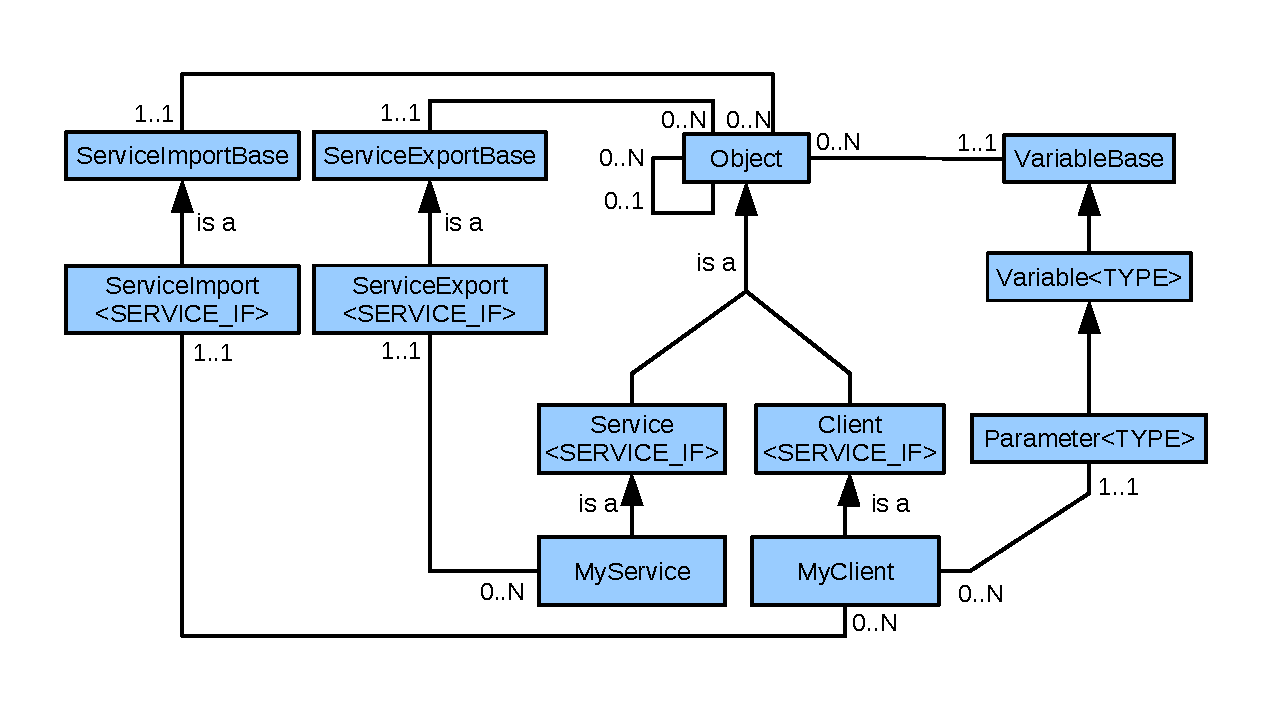
\includegraphics[width=\textwidth]{tms320c3x/fig_object_hierarchy.pdf}
	\end{center}
	\caption{Service/Client/Run-time Parameters Object hierarchy.}
	\label{fig:tms320c3x_object_hierarchy}
\end{figure}

\subsubsection{Building a service graph}
\label{tms320c3x_building_a_service_graph}

Using services implies building a service graph.
For instance, consider that the client is a loader, and the service is a memory.
The programmer creates objects \texttt{loader} and \texttt{memory}, see Figure~\ref{fig:tms320c3x_service_instanciation}.

\begin{figure}[h]
  \begin{center}
    \input{tms320c3x/service_instanciation}
    \caption{\label{fig:tms320c3x_service_instanciation} Client/Service instanciation.}
  \end{center}
\end{figure}

Object \texttt{loader} is a client because it needs a service (reading/writing in memory) from object \texttt{memory} to load the program.
\texttt{loader} has a member \texttt{import} named \texttt{memory\_import} whereas \texttt{memory} object has a member \texttt{export} named \texttt{memory\_export}.
The programmer connects the loader to the memory using \texttt{loader.memory\_import} and \texttt{memory.memory\_export}, see Figure~\ref{fig:tms320c3x_service_connection}.

\begin{figure}[h]
  \begin{center}
    \input{tms320c3x/service_connection}
    \caption{\label{fig:tms320c3x_service_connection} Import/Export connection.}
  \end{center}
\end{figure}

Once \hfill the \hfill programmer \hfill has \hfill created \hfill a \hfill service \hfill graph, \hfill he \hfill must \hfill perform \hfill a \hfill call \hfill to \hfill \texttt{ServiceManager::Setup()}.
\texttt{ServiceManager::Setup()} returns \texttt{true} if setup of each service and client in the graph has been successful, other it returns \texttt{false}.

\subsubsection{Designing a service}

A service is a C++ object inheriting from template class \texttt{Service<SERVICE\_INTERFACE>} \ding{202}, see Figure~\ref{fig:tms320c3x_simple_service}.
\texttt{SERVICE\_INTERFACE} is a C++ abstract class defining the virtual methods implemented by the service.
To export its interface, a service must have a member of type \texttt{ServiceExport<SERVICE\_INTERFACE>} \ding{203}.
For normalization purposes, the service constructor should take only two parameters \ding{204}: the service name and the pointer to the parent (a container service).
The pointer to the parent is \texttt{null} if the service is a top level service (no parent).
The base \texttt{Object} constructor \ding{205} and the base \texttt{Service} constructor \ding{206} must be called with the name and the pointer to the parent.
\texttt{ServiceExport} member constructor must be called with the export name and a pointer to the owner, i.e. the service itself \ding{207}.

\begin{figure}[h]
  \begin{center}
    \input{tms320c3x/simple_service}
    \caption{\label{fig:tms320c3x_simple_service} Simple service.}
  \end{center}
\end{figure}

\subsubsection{Designing a client}

A client is a C++ object inheriting from template class \texttt{Client<SERVICE\_INTERFACE>} \ding{202}, see Figure~\ref{fig:tms320c3x_simple_client}.
\texttt{SERVICE\_INTERFACE} is a C++ abstract class defining the virtual methods implemented by the service the client can call.
To import an interface, a client must have a member of type \texttt{ServiceImport<SERVICE\_INTERFACE>} \ding{203}.
For normalization purposes, the client constructor should take only two parameters \ding{204}: the client name and the pointer to the parent (a container client).
The pointer to the parent is \texttt{null} if the client is a top level client (no parent).
The base \texttt{Object} constructor \ding{205} and the base \texttt{Client} constructor \ding{206} must be called with the name and the pointer to the parent.
\texttt{ServiceImport} member constructor must be called with the import name and a pointer to the owner, i.e. the client itself \ding{207}.


\begin{figure}[h]
  \begin{center}
    \input{tms320c3x/simple_client}
    \caption{\label{fig:tms320c3x_simple_client} Simple client.}
  \end{center}
\end{figure}

\subsubsection{Run-time parameters}

Run-time parameterization can be added to a service or a client. "Run-time parametrization" means that the service and/or client can be reconfigured at run-time. It is opposed to "Static parametrization or template parametrization" which allows configuring a service and/or client at compilation-time.
To expose a member variable as a run-time parameter, a client/service must have member variable of type \texttt{Parameter<TYPE>}, where \texttt{TYPE} is the C++ type of the exposed member variable, see Figure~\ref{fig:tms320c3x_run_time_parameter}. Consider that a service would expose a member variable \texttt{x} \ding{202}. An instance of class \texttt{Parameter} is defined as a member of the service \ding{203}. 
The parameter is bound to the exposed variable \ding{204} in the service/client constructor.

\begin{figure}[h]
  \begin{center}
    \input{tms320c3x/run_time_parameter}
    \caption{\label{fig:tms320c3x_run_time_parameter} Exposing a service/client member variable as a run-time parameter.}
  \end{center}
\end{figure}

\subsubsection{Setup Order}

As explained in section~\ref{tms320c3x_building_a_service_graph}, Method \texttt{Setup} of class \texttt{ServiceManager} calls all \texttt{Setup} methods in the simulator. A problem may occur if setup order is important. For instance, consider two services: service \texttt{A} and \texttt{B}. \texttt{A::Setup()} uses service \texttt{B}. A correct setup order consist to first setup service \texttt{B} and then service \texttt{A}.
To solve such setup dependency, programmer should call method \texttt{Object::SetupDependsOn} (e.g. in the class constructor) so that the service manager can ensure correct setup order.
If the service manager finds a cyclic dependency, \texttt{ServiceManager::Setup()} fails: it generally means that clients and services have been badly designed.

\newpage
\subsection{Service Interfaces}
\label{tms320c3x_interfaces}

All service interfaces are declared in namespace \texttt{unisim::service::interfaces} and located in directory \texttt{unisim/service/interfaces}.

\subsubsection{Memory Interfaces}

These interfaces allows reading and writing to memory space. The memory interfaces comes in two flavor:
\begin{itemize}
\item non-instrusive memory access (\texttt{unisim::service::interfaces::Memory}); It should not affect timing and data placement (e.g. in caches and TLBs).
\item intrusive memory access (\texttt{unisim::service::interfaces::MemoryInjection}); It can affect timing and data placement.
\end{itemize}

\noindent The two C++ interfaces are:

\begin{center}
	\input{tms320c3x/memory_interface}
\end{center}

\begin{center}
	\input{tms320c3x/memory_injection_interface}
\end{center}

\noindent The arguments to methods \texttt{ReadMemory}, \texttt{InjectReadMemory}, \texttt{WriteMemory}, \texttt{InjectWriteMemory} are:
\begin{itemize}
\item \texttt{addr}: the starting address of the data transfer between the memory and the buffer
\item \texttt{buffer}: a pointer to the buffer of bytes
\item \texttt{size}: the length in bytes to transfer between the memory and the buffer
\end{itemize}

\subsubsection{Debugging Interfaces}

These interfaces are intended for interfacing simulation components (e.g. CPU, memory, devices, \ldots) with a debugger (e.g. inline-debugger, GDB server, \ldots).

\textbf{Instruction disassembly}. A CPU components provides a debugger with a disassembly capability of the instruction set using interface \texttt{unisim::service::interfaces::Disassembly}.

\begin{center}
	\input{tms320c3x/disassembly_interface}
\end{center}

\noindent Method \texttt{Disasm} arguments are:
\begin{itemize}
\item \texttt{addr}: the byte address of the instruction to disassemble
\item \texttt{next\_addr}: the byte address of the next instruction
\end{itemize}
\noindent and returns a string with the disassembly of the instruction.

\textbf{Register access}. A CPU or a device provides a debugger with an access to its registers using interface \texttt{unisim::service::interfaces::Registers}.

\begin{center}
	\input{tms320c3x/registers_interface}
\end{center}

\noindent Method \texttt{GetRegister} arguments are:
\begin{itemize}
\item \texttt{name}: the name of the register to retrieve interface
\end{itemize}
\noindent and returns a pointer to an interface \texttt{unisim::util::debug::Register}.

\begin{center}
	\input{tms320c3x/register_interface}
\end{center}

\noindent Method \texttt{GetName} returns the register name.
\noindent Method \texttt{GetValue} fills in a buffer with the register value.
\noindent Method \texttt{SetValue} sets the register value from a buffer.
\noindent Method \texttt{GetSize} returns the register size in bytes.

\textbf{Step by step execution}. A simulation component (e.g. a CPU) leaves control to a debugger with interface \texttt{unisim::service::interfaces::DebugControl}.

\begin{center}
	\input{tms320c3x/debug_control_interface}
\end{center}

Method \texttt{FetchDebugCommand} takes the current program counter as arguments and returns a command for the simulation component: either finish the simulation or execute one instruction.

\textbf{Monitoring memory accesses}. An instrumented simulation component provides a memory access trace using interface \texttt{unisim::service::interfaces::MemoryAccessReporting}.
Such memory trace is useful for a debugger to monitor memory access.

\begin{center}
	\input{tms320c3x/memory_access_reporting_interface}
\end{center}

Method \texttt{ReportMemoryAccess} takes as argument the memory access type (either read or write), the memory type (either data or instruction memory), the address of the access, and the size of the memory access.
Method \texttt{ReportFinishedInstruction} takes as argument the address of next instruction to be executed.

\textbf{Trap reporting}. An instrumented simulation component informs a debugger about an important event using interface \texttt{unisim::service::interfaces::TrapReporting}.
Such event is useful for a debugger to pause simulation once such event occurs.

\begin{center}
	\input{tms320c3x/trap_reporting_interface}
\end{center}

Method \texttt{ReportTrap} takes no arguments.

\textbf{Symbol}. A service (e.g. a loader) provides lookup to the symbol table using interface \texttt{unisim::service::interfaces::SymbolTableLookup}.
This interface is usefull for translating addresses to symbol names, and vice-versa.

\begin{center}
	\input{tms320c3x/symbol_table_lookup_interface}
\end{center}

\textbf{Efficient instrumentation.} To limit the impact on simulation performance of memory access instrumentation in the simulation components, such instrumentation can be enable or disable at run-time using interface \texttt{unisim::service::interfaces::MemoryAccessReportingControl}.

\begin{center}
	\input{tms320c3x/memory_access_reporting_control_interface}
\end{center}

\subsubsection{Loader Interface}

This interface provides basic informations about the loaded program.

\begin{center}
	\input{tms320c3x/loader_interface}
\end{center}

\subsubsection{Time Interface}

This interface provides reading of the current time.

\begin{center}
	\input{tms320c3x/time_interface}
\end{center}

\subsubsection{TI C I/O Interface}

An instrumented TMS320C3X instruction set simulator provides a trace of \texttt{SWI} instructions using interface \texttt{unisim::service::interfaces::ti\_c\_io}.
This interface is useful for the TI C I/O service to capture target program I/Os and translate them to host I/Os.

\begin{center}
	\input{tms320c3x/ti_c_io_interface}
\end{center}

\newpage
\subsection{Services}
\subsubsection{COFF loader service}
\label{tms320c3x_coff_loader}

This service provides UNISIM TMS320C3X simulator with a support for TI COFF v0, v1, and v2 binary files (see TMS320C3x/C4x Assembly Language Tools User’s Guide, Appendix A). The COFF loader service loads the programs into memory while setup (simulator initialization). The loader can interprete \texttt{.cinit} section if option \texttt{-cr} of TI C cross-compiler has been used while building the target program (see TMS320C3x/C4x Optimizing C Compiler User’s Guide, section 4.8.1: Autoinitialization of variables and constants).
To configure the COFF loader service see section~\ref{tms320c3x_configuration}.
The source code of COFF loader service is located in directory \texttt{unisim/service/loader/coff\_loader}.
\noindent Table below summarizes the COFF Loader service API:

\begin{center}
	\tablehead{\hline}
	\tabletail{\hline}
	\begin{supertabular}{|p{7.5cm}|p{7.5cm}|}
		\hline
		\multicolumn{2}{|l|}{\textbf{\Large Service COFF Loader}}\\
		\hline
		\multicolumn{1}{|p{7.5cm}}{\textbf{Class Name:} \newline \texttt{unisim::service::loader::coff\_loader}\newline$\hookrightarrow$\texttt{::CoffLoader}} & \multicolumn{1}{p{7.5cm}|}{\textbf{Header:} \newline \texttt{unisim/service/loader/coff\_loader}\newline$\hookrightarrow$\texttt{/coff\_loader.hh}}\\
		\multicolumn{2}{|l|}{}\\
		\multicolumn{2}{|p{15cm}|}{\textbf{Description:} \newline The COFF loader service allows to load a COFF binary program into a memory and fill a symbol table. The loader also provides information about the loaded file such as the code and data locations (base address and size). The COFF loader loads the program during setup.}\\
		\hline
		\hline
		\multicolumn{2}{|c|}{\textbf{\large Template Parameters}}\\
		\hline
		\multicolumn{1}{|p{7.5cm}}{\textbf{Name:} \texttt{MEMORY\_ADDR}} & \multicolumn{1}{p{7.5cm}|}{\textbf{Type:} \texttt{class}}\\
		\multicolumn{2}{|p{15cm}|}{\textbf{Default value:} \texttt{none}}\\
		\multicolumn{2}{|l|}{}\\
		\multicolumn{2}{|p{15cm}|}{\textbf{Description:} \newline This is the C++ type of a memory address (e.g. \texttt{uint32\_t} or \texttt{uint64\_t}).}\\
		\hline
		\hline
		\multicolumn{2}{|c|}{\textbf{\large Run-Time Parameters}}\\
		\hline
		\multicolumn{1}{|p{7.5cm}}{\textbf{Name:} \texttt{filename}} & \multicolumn{1}{p{7.5cm}|}{\textbf{Type:} \texttt{string}}\\
		\multicolumn{2}{|p{15cm}|}{\textbf{Default value:} empty string}\\
		\multicolumn{2}{|l|}{}\\
		\multicolumn{2}{|p{15cm}|}{\textbf{Description:} \newline The COFF file name to load into the connected memory.}\\
		\hline
		\hline
		\multicolumn{1}{|p{7.5cm}}{\textbf{Name:} \texttt{dump-headers}} & \multicolumn{1}{p{7.5cm}|}{\textbf{Type:} \texttt{boolean}}\\
		\multicolumn{2}{|p{15cm}|}{\textbf{Default value:} false}\\
		\multicolumn{2}{|l|}{}\\
		\multicolumn{2}{|p{15cm}|}{\textbf{Description:} \newline If true this parameter makes the COFF loader print the file headers on the screen (file header, section headers, symbol table \ldots) while loading the program.}\\
		\hline
		\multicolumn{2}{|c|}{\textbf{\large Service Exports}}\\
		\hline
		\multicolumn{1}{|p{7.5cm}}{\textbf{Name:} \texttt{logger\_export}} & \multicolumn{1}{p{7.5cm}|}{\textbf{Interface:} \newline \texttt{unisim::service::interfaces::} \newline$\hookrightarrow$\texttt{Loader<MEMORY\_ADDR>}}\\
		\multicolumn{2}{|l|}{}\\
		\multicolumn{2}{|p{15cm}|}{\textbf{Description:} \newline The COFF loader provides information about the code and data location through this export.}\\
		\hline
		\multicolumn{1}{|p{7.5cm}}{\textbf{Name:} \texttt{symbol\_table\_lookup\_export}} & \multicolumn{1}{p{7.5cm}|}{\textbf{Interface:} \newline \texttt{unisim::service::interfaces::} \newline$\hookrightarrow$\texttt{SymbolTableLookup<MEMORY\_ADDR>}}\\
		\multicolumn{2}{|l|}{}\\
		\multicolumn{2}{|p{15cm}|}{\textbf{Description:} \newline The COFF loader provides symbol lookup through this export.}\\
		\hline
		\hline
		\multicolumn{2}{|c|}{\textbf{\large Service Imports}}\\
		\hline
		\multicolumn{1}{|p{7.5cm}}{\textbf{Name:} \texttt{memory\_import} \newline \textbf{Mandatory connected:} no} & \multicolumn{1}{p{7.5cm}|}{\textbf{Interface:} \newline \texttt{unisim::service::interfaces::} \newline$\hookrightarrow$\texttt{Memory<uint32\_t>}}\\
		\multicolumn{2}{|l|}{}\\
		\multicolumn{2}{|p{15cm}|}{\textbf{Description:} \newline The COFF loader accesses to the memory through this import.}\\
		\hline
	\end{supertabular}
\end{center}

\newpage
\subsubsection{TI C I/O service}
\label{tms320c3x_ti_c_io}

This service provides target programs with a support for low level I/O (open, read, write, close, \ldots) on the host machine.
The TI Run-time support libraries (\texttt{RTS*.lib}) implements a software stack for standard C I/Os (see TMS320C3x/C4x Optimizing C Compiler User’s Guide (SPRU034H, June 1998), Appendix B).
A development board debugger captures target program I/Os at \texttt{C\$\$IO\$\$}. The Run-time support library puts the I/Os in a communication buffer (\texttt{\_\_CIOBUF\_}) that the development board debugger translates to host I/Os. The debugger also captures target program termination at \texttt{C\$\$EXIT}.
The UNISIM TI C I/O service captures and translates target program I/Os and termination in same manner as a development board built-in debugger.
To configure the TI C I/O service see section~\ref{tms320c3x_configuration}.
The source code of COFF loader service is located in directory \texttt{unisim/service/os/ti\_c\_io}.
\noindent Table below summarizes the TI C I/O service API:

\begin{center}
	\tablehead{\hline}
	\tabletail{\hline}
	\begin{supertabular}{|p{7.5cm}|p{7.5cm}|}
		\hline
		\multicolumn{2}{|l|}{\textbf{\Large Service TI C I/O}}\\
		\hline
		\multicolumn{1}{|p{7.5cm}}{\textbf{Class Name:} \newline \texttt{unisim::service::os::ti\_c\_io}\newline$\hookrightarrow$\texttt{::TI\_C\_IO}} & \multicolumn{1}{p{7.5cm}|}{\textbf{Header:} \newline \texttt{unisim/service/os/ti\_c\_io}\newline$\hookrightarrow$\texttt{/ti\_c\_io.hh}}\\
		\multicolumn{2}{|l|}{}\\
		\multicolumn{2}{|p{15cm}|}{\textbf{Description:} \newline The TI C I/O service provides target programs with a support for low level I/O (open, read, write, close, \ldots) on the host machine.}\\
		\hline
		\hline
		\multicolumn{2}{|c|}{\textbf{\large Template Parameters}}\\
		\hline
		\multicolumn{1}{|p{7.5cm}}{\textbf{Name:} \texttt{MEMORY\_ADDR}} & \multicolumn{1}{p{7.5cm}|}{\textbf{Type:} \texttt{class}}\\
		\multicolumn{2}{|p{15cm}|}{\textbf{Default value:} \texttt{none}}\\
		\multicolumn{2}{|l|}{}\\
		\multicolumn{2}{|p{15cm}|}{\textbf{Description:} \newline This is the C++ type of a memory address (e.g. uint32\_t or uint64\_t).}\\
		\hline
		\hline
		\multicolumn{2}{|c|}{\textbf{\large Run-Time Parameters}}\\
		\hline
		\multicolumn{1}{|p{7.5cm}}{\textbf{Name:} \texttt{ti\_c\_io.enable}} & \multicolumn{1}{p{7.5cm}|}{\textbf{Type:} \texttt{bool}}\\
		\multicolumn{2}{|p{15cm}|}{\textbf{Default value:} \texttt{false}}\\
		\multicolumn{2}{|l|}{}\\
		\multicolumn{2}{|p{15cm}|}{\textbf{Description:} \newline Enable/Disable TI C I/O support.}\\
		\hline
		\multicolumn{1}{|p{7.5cm}}{\textbf{Name:} \texttt{ti-c-io.warning-as-error}} & \multicolumn{1}{p{7.5cm}|}{\textbf{Type:} \texttt{bool}}\\
		\multicolumn{2}{|p{15cm}|}{\textbf{Default value:} \texttt{false}}\\
		\multicolumn{2}{|l|}{}\\
		\multicolumn{2}{|p{15cm}|}{\textbf{Description:} \newline Whether Warnings are considered as error or not.}\\
		\hline
		\multicolumn{1}{|p{7.5cm}}{\textbf{Name:} \texttt{ti-c-io.pc-register-name}} & \multicolumn{1}{p{7.5cm}|}{\textbf{Type:} \texttt{string}}\\
		\multicolumn{2}{|p{15cm}|}{\textbf{Default value:} \texttt{"PC"}}\\
		\multicolumn{2}{|l|}{}\\
		\multicolumn{2}{|p{15cm}|}{\textbf{Description:} \newline Name of the CPU program counter register.}\\
		\hline
		\multicolumn{1}{|p{7.5cm}}{\textbf{Name:} \texttt{ti-c-io.c-io-buffer-symbol-name}} & \multicolumn{1}{p{7.5cm}|}{\textbf{Type:} \texttt{string}}\\
		\multicolumn{2}{|p{15cm}|}{\textbf{Default value:} \texttt{"\_\_CIOBUF\_"}}\\
		\multicolumn{2}{|l|}{}\\
		\multicolumn{2}{|p{15cm}|}{\textbf{Description:} \newline C I/O buffer symbol name.}\\
		\hline
		\multicolumn{1}{|p{7.5cm}}{\textbf{Name:} \texttt{ti-c-io.c-io-breakpoint-}\newline$\hookrightarrow$\texttt{symbol-name}} & \multicolumn{1}{p{7.5cm}|}{\textbf{Type:} \texttt{string}}\\
		\multicolumn{2}{|p{15cm}|}{\textbf{Default value:} \texttt{"C\$\$IO\$\$"}}\\
		\multicolumn{2}{|l|}{}\\
		\multicolumn{2}{|p{15cm}|}{\textbf{Description:} \newline C I/O breakpoint symbol name. The TI C I/O service installs an \texttt{SWI} instruction at this point to capture target program I/O.}\\
		\hline
		\multicolumn{1}{|p{7.5cm}}{\textbf{Name:} \texttt{ti-c-io.c-exit-breakpoint-}\newline$\hookrightarrow$\texttt{symbol-name}} & \multicolumn{1}{p{7.5cm}|}{\textbf{Type:} \texttt{string}}\\
		\multicolumn{2}{|p{15cm}|}{\textbf{Default value:} \texttt{"C\$\$EXIT"}}\\
		\multicolumn{2}{|l|}{}\\
		\multicolumn{2}{|p{15cm}|}{\textbf{Description:} \newline C EXIT breakpoint symbol name. The TI C I/O service installs an \texttt{SWI} instruction at this point to capture target program exit.}\\
		\hline
		\multicolumn{1}{|p{7.5cm}}{\textbf{Name:} \texttt{ti-c-io.verbose-all}} & \multicolumn{1}{p{7.5cm}|}{\textbf{Type:} \texttt{bool}}\\
		\multicolumn{2}{|p{15cm}|}{\textbf{Default value:} \texttt{false}}\\
		\multicolumn{2}{|l|}{}\\
		\multicolumn{2}{|p{15cm}|}{\textbf{Description:} \newline Globally enable/disable verbosity of TI C I/O service.}\\
		\hline
		\multicolumn{1}{|p{7.5cm}}{\textbf{Name:} \texttt{ti-c-io.verbose-io}} & \multicolumn{1}{p{7.5cm}|}{\textbf{Type:} \texttt{bool}}\\
		\multicolumn{2}{|p{15cm}|}{\textbf{Default value:} \texttt{false}}\\
		\multicolumn{2}{|l|}{}\\
		\multicolumn{2}{|p{15cm}|}{\textbf{Description:} \newline Enable/disable verbosity of TI C I/O service while I/Os.}\\
		\hline
		\multicolumn{1}{|p{7.5cm}}{\textbf{Name:} \texttt{ti-c-io.verbose-setup}} & \multicolumn{1}{p{7.5cm}|}{\textbf{Type:} \texttt{bool}}\\
		\multicolumn{2}{|p{15cm}|}{\textbf{Default value:} \texttt{false}}\\
		\multicolumn{2}{|l|}{}\\
		\multicolumn{2}{|p{15cm}|}{\textbf{Description:} \newline Enable/disable verbosity of TI C I/O service while setup.}\\
		\hline
		\hline
		\multicolumn{2}{|c|}{\textbf{\large Service Exports}}\\
		\hline
		\multicolumn{1}{|p{7.5cm}}{\textbf{Name:} \texttt{ti\_c\_io\_export}} & \multicolumn{1}{p{7.5cm}|}{\textbf{Interface:} \newline \texttt{unisim::interfaces::} \newline$\hookrightarrow$\texttt{TI\_C\_IO<MEMORY\_ADDR>}}\\
		\multicolumn{2}{|l|}{}\\
		\multicolumn{2}{|p{15cm}|}{\textbf{Description:} \newline The TI C I/O provides target to host I/O translation through this service export.}\\
		\hline
		\hline
		\multicolumn{2}{|c|}{\textbf{\large Service Imports}}\\
		\hline
		\multicolumn{1}{|p{7.5cm}}{\textbf{Name:} \texttt{memory\_import}} & \multicolumn{1}{p{7.5cm}|}{\textbf{Interface:} \newline \texttt{unisim::service::interfaces::} \newline$\hookrightarrow$\texttt{Memory<MEMORY\_ADDR>}}\\
		\multicolumn{2}{|p{15cm}|}{\textbf{Mandatory connected:} no}\\
		\multicolumn{2}{|l|}{}\\
		\multicolumn{2}{|p{15cm}|}{\textbf{Description:} \newline The TI C I/O service accesses to the memory while setup through this import. While setup it installs a two \texttt{SWI} instructions to capture both target I/O and program exit.}\\
		\hline
		\multicolumn{1}{|p{7.5cm}}{\textbf{Name:} \texttt{memory\_injection\_import}} & \multicolumn{1}{p{7.5cm}|}{\textbf{Interface:} \newline \texttt{unisim::service::interfaces::} \newline$\hookrightarrow$\texttt{MemoryInjection<MEMORY\_ADDR>}}\\
		\multicolumn{2}{|p{15cm}|}{\textbf{Mandatory connected:} no}\\
		\multicolumn{2}{|l|}{}\\
		\multicolumn{2}{|p{15cm}|}{\textbf{Description:} \newline The TI C I/O service accesses to the memory while simulation through this import. It accesses to the I/O buffer in the target program memory and then interprete the content of this buffer to translate target program I/Os to host I/Os.}\\
		\hline
		\multicolumn{1}{|p{7.5cm}}{\textbf{Name:} \texttt{registers\_import} \newline \textbf{Mandatory connected:} yes} & \multicolumn{1}{p{7.5cm}|}{\textbf{Interface:} \newline \texttt{unisim::service::interfaces} \newline$\hookrightarrow$\texttt{::Registers}}\\
		\multicolumn{2}{|l|}{}\\
		\multicolumn{2}{|p{15cm}|}{\textbf{Description:} \newline This service import should be connected to a CPU module. The TI C I/O service calls method \texttt{GetRegister} through this service import to get an interface to the CPU registers. The TI C I/O service uses methods \texttt{GetName}, \texttt{GetValue}, \texttt{GetSize} and \texttt{SetValue} of that interface to access to CPU registers. This import is mainly used to get the current PC, so that the TI C I/O service can distinguish target program I/Os from target program exit.}\\
		\hline
		\multicolumn{1}{|p{7.5cm}}{\textbf{Name:} \texttt{symbol\_table\_lookup\_import} \newline \textbf{Mandatory connected:} yes} & \multicolumn{1}{p{7.5cm}|}{\textbf{Interface:} \newline \texttt{unisim::service::interfaces} \newline$\hookrightarrow$\texttt{::SymbolTableLookup<MEMORY\_ADDR>}}\\
		\multicolumn{2}{|l|}{}\\
		\multicolumn{2}{|p{15cm}|}{\textbf{Description:} \newline The TI C I/O service uses this service import get the address of the breakpoints and I/O buffer from their symbol name.}\\
		\hline
	\end{supertabular}
\end{center}

\newpage
\subsubsection{Inline debugger}
\label{tms320c3x_inline_debugger}

The inline debugger service is a built-in debugger with a text-based user interface, see~\ref{tms320c3x_inline_debug}. It provides instruction level debugging of the target program.
\noindent Table below summarizes the inline debugger service API:

\begin{center}
	\tablehead{\hline}
	\tabletail{\hline}
	\begin{supertabular}{|p{7.5cm}|p{7.5cm}|}
		\hline
		\multicolumn{2}{|l|}{\textbf{\Large Service Inline Debugger}}\\
		\hline
		\multicolumn{1}{|p{7.5cm}}{\textbf{Class Name:} \newline \texttt{unisim::service::debug}\newline$\hookrightarrow$\texttt{::inline\_debugger::InlineDebugger}} & \multicolumn{1}{p{7.5cm}|}{\textbf{Header:} \newline \texttt{unisim/service/debug}\newline$\hookrightarrow$\texttt{/inline\_debugger/inline\_debugger.hh}}\\
		\multicolumn{2}{|l|}{}\\
		\multicolumn{2}{|p{15cm}|}{\textbf{Description:} \newline The inline debugger service provides the user with a simple text-based interface to interactively debug a target application running on a CPU module. The debug is at the instruction level. The inline debugger may be connected to a CPU module.}\\
		\hline
		\hline
		\multicolumn{2}{|c|}{\textbf{\large Template Parameters}}\\
		\hline
		\multicolumn{1}{|p{7.5cm}}{\textbf{Name:} \texttt{ADDRESS}} & \multicolumn{1}{p{7.5cm}|}{\textbf{Type:} \texttt{class}}\\
		\multicolumn{2}{|p{15cm}|}{\textbf{Default value:} none}\\
		\multicolumn{2}{|l|}{}\\
		\multicolumn{2}{|p{15cm}|}{\textbf{Description:} \newline This is the C++ type of a memory address (e.g. uint32\_t or uint64\_t).}\\
		\hline
		\hline
		\multicolumn{2}{|c|}{\textbf{\large Run-time parameters}}\\
		\hline
		\multicolumn{1}{|p{7.5cm}}{\textbf{Name:} \texttt{inline-debugger.memory-atom-size}} & \multicolumn{1}{p{7.5cm}|}{\textbf{Type:} \texttt{unsigned integer}}\\
		\multicolumn{2}{|p{15cm}|}{\textbf{Default value:} \texttt{1}}\\
		\multicolumn{2}{|l|}{}\\
		\multicolumn{2}{|p{15cm}|}{\textbf{Description:} \newline Size of the smallest addressable element in memory.}\\
		\hline
		\hline
		\multicolumn{2}{|c|}{\textbf{\large Service Exports}}\\
		\hline
		\multicolumn{1}{|p{7.5cm}}{\textbf{Name:} \texttt{debug\_control\_export}} & \multicolumn{1}{p{7.5cm}|}{\textbf{Interface:} \newline \texttt{unisim::service::interfaces} \newline$\hookrightarrow$\texttt{::DebugControl<ADDRESS>}}\\
		\multicolumn{2}{|l|}{}\\
		\multicolumn{2}{|p{15cm}|}{\textbf{Description:} \newline This service export should be connected to a CPU module. The CPU module calls method \texttt{FetchDebugCommand} through its service import to leave control to the debugger and fetch a new debug command.}\\
		\hline
		\multicolumn{1}{|p{7.5cm}}{\textbf{Name:} \texttt{memory\_access\_reporting\_export}} & \multicolumn{1}{p{7.5cm}|}{\textbf{Interface:} \newline \texttt{unisim::service::interfaces} \newline$\hookrightarrow$\texttt{MemoryAccessReporting<ADDRESS>}}\\
		\multicolumn{2}{|l|}{}\\
		\multicolumn{2}{|p{15cm}|}{\textbf{Description:} \newline This service export should be connected to a CPU module. The CPU module calls methods \texttt{ReportMemoryAccess} and \texttt{ReportFinishedInstruction} through its service import. This allows the debugger to spy memory accesses and thus handle breakpoints and watchpoints.}\\
		\hline
		\multicolumn{1}{|p{7.5cm}}{\textbf{Name:} \texttt{trap\_reporting\_export}} & \multicolumn{1}{p{7.5cm}|}{\textbf{Interface:} \newline \texttt{unisim::service::interfaces} \newline$\hookrightarrow$\texttt{::TrapReporting}}\\
		\multicolumn{2}{|l|}{}\\
		\multicolumn{2}{|p{15cm}|}{\textbf{Description:} \newline This service export should be connected to a CPU module. A CPU module calls method \texttt{ReportTrap} through its service import. This allows the debugger to break execution on the simulated CPU once a trap condition is detected by the CPU module.}\\
		\hline
		\hline
		\multicolumn{2}{|c|}{\textbf{\large Service Imports}}\\
		\hline
		\multicolumn{1}{|p{7.5cm}}{\textbf{Name:} \texttt{disasm\_import} \newline \textbf{Mandatory connected:} yes} & \multicolumn{1}{p{7.5cm}|}{\textbf{Interface:} \newline \texttt{unisim::service::interfaces} \newline$\hookrightarrow$\texttt{::Disassembly<ADDRESS>}}\\
		\multicolumn{2}{|l|}{}\\
		\multicolumn{2}{|p{15cm}|}{\textbf{Description:} \newline This service import should be connected to a CPU module. The CPU module should implements method \texttt{Disassemble} which provides the debugger with disassembling of the instructions.}\\
		\hline
		\multicolumn{1}{|p{7.5cm}}{\textbf{Name:} \texttt{memory\_import} \newline \textbf{Mandatory connected:} yes} & \multicolumn{1}{p{7.5cm}|}{\textbf{Interface:} \newline \texttt{unisim::service::interfaces} \newline$\hookrightarrow$\texttt{::Memory<ADDRESS>}}\\
		\multicolumn{2}{|l|}{}\\
		\multicolumn{2}{|p{15cm}|}{\textbf{Description:} \newline This service import should be connected to a CPU or a memory module. The debugger uses this service import to access to memory using methods \texttt{ReadMemory} and \texttt{WriteMemory}.}\\
		\hline
		\multicolumn{1}{|p{7.5cm}}{\textbf{Name:} \texttt{memory\_access\_reporting\newline$\hookrightarrow$\_control\_import} \newline \textbf{Mandatory connected:} no} & \multicolumn{1}{p{7.5cm}|}{\textbf{Interface:} \newline \texttt{unisim::service::interfaces} \newline$\hookrightarrow$\texttt{::MemoryAccessReportingControl}}\\
		\multicolumn{2}{|l|}{}\\
		\multicolumn{2}{|p{15cm}|}{\textbf{Description:} \newline This service import should be connected to a CPU module. The debugger calls methods \texttt{RequiresMemoryAccessReporting} and \texttt{RequiresFinishedInstructionReporting} through this service import to enable/disable memory access reporting from the CPU module.}\\
		\hline
		\multicolumn{1}{|p{7.5cm}}{\textbf{Name:} \texttt{registers\_import} \newline \textbf{Mandatory connected:} yes} & \multicolumn{1}{p{7.5cm}|}{\textbf{Interface:} \newline \texttt{unisim::service::interfaces} \newline$\hookrightarrow$\texttt{::Registers}}\\
		\multicolumn{2}{|l|}{}\\
		\multicolumn{2}{|p{15cm}|}{\textbf{Description:} \newline This service import should be connected to a CPU module. The debugger calls method \texttt{GetRegister} through this service import to get an interface to the CPU registers. The debugger uses methods \texttt{GetName}, \texttt{GetValue}, \texttt{GetSize} and \texttt{SetValue} of that interface to access to CPU registers.}\\
		\hline
		\multicolumn{1}{|p{7.5cm}}{\textbf{Name:} \texttt{symbol\_table\_lookup\_import} \newline \textbf{Mandatory connected:} no} & \multicolumn{1}{p{7.5cm}|}{\textbf{Interface:} \newline \texttt{unisim::service::interfaces} \newline$\hookrightarrow$\texttt{::SymbolTableLookup}}\\
		\multicolumn{2}{|l|}{}\\
		\multicolumn{2}{|p{15cm}|}{\textbf{Description:} \newline This service import should be connected to a symbol table. The debugger calls method \texttt{FindSymbol}, \texttt{FindSymbolByAddr}, \texttt{FindSymbolByName} through this service import to translate address to symbol and vice-versa.}\\
		\hline
	\end{supertabular}
\end{center}

\newpage
\subsubsection{GDB server}
\label{tms320c3x_gdb_server}

The GDB server service emulates the GDB remote serial protocol over TCP/IP (see Debugging with GDB, Appendix D. GDB Remote serial protocol), so that a GDB client can connect to the simulator and debug the target program as if it were run on the real hardware.
This service uses an architecture XML description file defined by the \texttt{architecture-description-filename} run-time parameter (see table below).
A sample configuration file for a dummy \texttt{XYZ} big-endian architecture, with four 32-bit general purpose registers named \texttt{r0}, \texttt{r1}, \texttt{r2}, \texttt{r3} and a program counter named \texttt{pc} would be the following:
\begin{verbatim}
<architecture name="XYZ" endian="big">
    <program_counter name="pc"/>
    <register name="r0" size="4"/>
    <register name="r1" size="4"/>
    <register name="r2" size="4"/>
    <register name="r3" size="4"/>
</architecture>
\end{verbatim}

\noindent Table below summarizes the GDB server service API:

\begin{center}
	\tablehead{\hline}
	\tabletail{\hline}
	\begin{supertabular}{|p{7.5cm}|p{7.5cm}|}
		\hline
		\multicolumn{2}{|l|}{\textbf{\Large Service GDB Server}}\\
		\hline
		\multicolumn{1}{|p{7.5cm}}{\textbf{Class Name:} \newline \texttt{unisim::service::debug}\newline$\hookrightarrow$\texttt{::gdb\_server::GDBServer}} & \multicolumn{1}{p{7.5cm}|}{\textbf{Header:} \newline \texttt{unisim/service/debug}\newline$\hookrightarrow$\texttt{/gdb\_server/gdb\_server.hh}}\\
		\multicolumn{2}{|l|}{}\\
		\multicolumn{2}{|p{15cm}|}{\textbf{Description:} \newline The GDB server service allows debugging a software running on a simulated hardware by connecting (over TCP/IP) a GDB client to it (and thus to the simulator). The GDB client can be either the standard text based client (i.e. command \texttt{gdb}), a graphical front-end to GDB (e.g. \texttt{ddd}), or even Eclipse CDT. The GDB server service directly speaks the GDB serial remote protocol (over TCP/IP), so that a GDB client can connect (over TCP/IP) to the simulator using GDB command \texttt{target remote}. The GDB server service may be connected to a CPU module.}\\
		\hline
		\hline
		\multicolumn{2}{|c|}{\textbf{\large Template Parameters}}\\
		\hline
		\multicolumn{1}{|p{7.5cm}}{\textbf{Name:} \texttt{ADDRESS}} & \multicolumn{1}{p{7.5cm}|}{\textbf{Type:} \texttt{class}}\\
		\multicolumn{2}{|p{15cm}|}{\textbf{Default value:} none}\\
		\multicolumn{2}{|l|}{}\\
		\multicolumn{2}{|p{15cm}|}{\textbf{Description:} \newline This is the C++ type of a memory address (e.g. uint32\_t or uint64\_t).}\\
		\hline
		\hline
		\multicolumn{2}{|c|}{\textbf{\large Run-Time Parameters}}\\
		\hline
		\multicolumn{1}{|p{7.5cm}}{\textbf{Name:} \texttt{tcp-port}} & \multicolumn{1}{p{7.5cm}|}{\textbf{Type:} \texttt{int}}\\
		\multicolumn{2}{|p{15cm}|}{\textbf{Default value:} \texttt{12345}}\\
		\multicolumn{2}{|l|}{}\\
		\multicolumn{2}{|p{15cm}|}{\textbf{Description:} \newline The TCP port used by GDB server service to communicate with the GDB client.}\\
		\hline
		\multicolumn{1}{|p{7.5cm}}{\textbf{Name:} \texttt{architecture-description\newline$\hookrightarrow$-filename}} & \multicolumn{1}{p{7.5cm}|}{\textbf{Type:} \texttt{string}}\\
		\multicolumn{2}{|p{15cm}|}{\textbf{Default value:} empty string}\\
		\multicolumn{2}{|l|}{}\\
		\multicolumn{2}{|p{15cm}|}{\textbf{Description:} \newline The path to the architecture description file that the GDB server service must use. The description file provides retargetability to the GDB server service. The following files brings support of the ARM, PowerPC and HCS12X processors to the GDB server service: 
		\begin{itemize}
			\item \texttt{unisim/service/debug/gdb\_server/gdb\_armv4l.xml}
			\item \texttt{unisim/service/debug/gdb\_server/gdb\_armv5b.xml}
			\item \texttt{unisim/service/debug/gdb\_server/gdb\_powerpc.xml}
			\item \texttt{unisim/service/debug/gdb\_server/gdb\_hcs12x.xml}
		\end{itemize}
		}\\
		\hline
		\hline
		\multicolumn{2}{|c|}{\textbf{\large Service Exports}}\\
		\hline
		\multicolumn{1}{|p{7.5cm}}{\textbf{Name:} \texttt{debug\_control\_export}} & \multicolumn{1}{p{7.5cm}|}{\textbf{Interface:} \newline \texttt{unisim::service::interfaces} \newline$\hookrightarrow$\texttt{::DebugControl<ADDRESS>}}\\
		\multicolumn{2}{|l|}{}\\
		\multicolumn{2}{|p{15cm}|}{\textbf{Description:} \newline This service export should be connected to a CPU module. The CPU module calls method \texttt{FetchDebugCommand} through its service import to leave control to the debugger and fetch a new debug command.}\\
		\hline
		\multicolumn{1}{|p{7.5cm}}{\textbf{Name:} \texttt{memory\_access\_reporting\_export}} & \multicolumn{1}{p{7.5cm}|}{\textbf{Interface:} \newline \texttt{unisim::service::interfaces} \newline$\hookrightarrow$\texttt{MemoryAccessReporting<ADDRESS>}}\\
		\multicolumn{2}{|l|}{}\\
		\multicolumn{2}{|p{15cm}|}{\textbf{Description:} \newline This service export should be connected to a CPU module. The CPU module calls methods \texttt{ReportMemoryAccess} and \texttt{ReportFinishedInstruction} through its service import. This allows the debugger to spy memory accesses and thus handle breakpoints and watchpoints.}\\
		\hline
		\multicolumn{1}{|p{7.5cm}}{\textbf{Name:} \texttt{trap\_reporting\_export}} & \multicolumn{1}{p{7.5cm}|}{\textbf{Interface:} \newline \texttt{unisim::service::interfaces} \newline$\hookrightarrow$\texttt{::TrapReporting}}\\
		\multicolumn{2}{|l|}{}\\
		\multicolumn{2}{|p{15cm}|}{\textbf{Description:} \newline This service export should be connected to a CPU module. A CPU module calls method \texttt{ReportTrap} through its service import. This allows the debugger to break execution on the simulated CPU once a trap condition is detected by the CPU module.}\\
		\hline
		\hline
		\multicolumn{2}{|c|}{\textbf{\large Service Imports}}\\
		\hline
		\multicolumn{1}{|p{7.5cm}}{\textbf{Name:} \texttt{memory\_import} \newline \textbf{Mandatory connected:} yes} & \multicolumn{1}{p{7.5cm}|}{\textbf{Interface:} \newline \texttt{unisim::service::interfaces} \newline$\hookrightarrow$\texttt{::Memory<ADDRESS>}}\\
		\multicolumn{2}{|l|}{}\\
		\multicolumn{2}{|p{15cm}|}{\textbf{Description:} \newline This service import should be connected to a CPU or a memory module. The debugger uses this service import to access to memory using methods \texttt{ReadMemory} and \texttt{WriteMemory}.}\\
		\hline
		\multicolumn{1}{|p{7.5cm}}{\textbf{Name:} \texttt{memory\_access\_reporting\newline$\hookrightarrow$\_control\_import} \newline \textbf{Mandatory connected:} no} & \multicolumn{1}{p{7.5cm}|}{\textbf{Interface:} \newline \texttt{unisim::service::interfaces} \newline$\hookrightarrow$\texttt{::MemoryAccessReportingControl}}\\
		\multicolumn{2}{|l|}{}\\
		\multicolumn{2}{|p{15cm}|}{\textbf{Description:} \newline This service import should be connected to a CPU module. The debugger calls methods \texttt{RequiresMemoryAccessReporting} and \texttt{RequiresFinishedInstructionReporting} through this service import to enable/disable memory access reporting from the CPU module.}\\
		\hline
		\multicolumn{1}{|p{7.5cm}}{\textbf{Name:} \texttt{registers\_import} \newline \textbf{Mandatory connected:} yes} & \multicolumn{1}{p{7.5cm}|}{\textbf{Interface:} \newline \texttt{unisim::service::interfaces} \newline$\hookrightarrow$\texttt{::Registers}}\\
		\multicolumn{2}{|l|}{}\\
		\multicolumn{2}{|p{15cm}|}{\textbf{Description:} \newline This service import should be connected to a CPU module. The debugger calls method \texttt{GetRegister} through this service import to get an interface to the CPU registers. The debugger uses methods \texttt{GetName}, \texttt{GetValue}, \texttt{GetSize} and \texttt{SetValue} of that interface to access to CPU registers.}\\
		\hline
	\end{supertabular}
\end{center}

\newpage
\subsubsection{Built-in Logger}
\label{tms320c3x_logger}

UNISIM provides you a centralized log system to debug modules and simulators. It should be used to show all debug messages, instead of using the traditional C++ stream output mechanism (\texttt{cerr} and \texttt{cout}). However, as you will see below the UNISIM log system works much like the C++ stream output mechanism.

It provides the following advantages:
\begin{itemize}
\item Categorization: messages can be categorized on information, warning and error messages
\item Atomic messages: messages will not be mixed (something which happens when programming concurrent/parallel systems like UNISIM/SystemC)
\item Multiple outputs: your messages can be written simultaneously to different outputs, for example:
	\begin{itemize}
	\item console (error output or standard output)
	\item raw file
	\item XML formatted file
	\item ...
	\end{itemize}
\item Simple configuration: the log system configuration is integrated to the UNISIM parameter mechanism provided by UNISIM service, see~\ref{tms320c3x_configuration}.
\end{itemize}

To use the UNISIM logger you need to include “unisim/kernel/logger/logger.hh” and declare that you are using the unisim::kernel::logger namespace:

\begin{center}
	\input{tms320c3x/including_logger}
\end{center}

The logger can only be used by UNISIM Objects, that is, classes that inherit from \newline
\texttt{unisim::kernel::service::Object}. So if you want to use the UNISIM log system your class must inherit from a UNISIM Object.

\begin{center}
	\input{tms320c3x/deriving_from_object}
\end{center}

You will need to create a member variable of the \texttt{unisim::kernel::logger::Logger} type. And at the construction of your object use its default constructor \newline
\texttt{Logger(const unisim::kernel::service::Object \&obj)}. For example:

\begin{center}
	\input{tms320c3x/binding_logger}
\end{center}

Once you have initialized your member logger variable you can start using it in your class methods. Basically it works like an standard C++ output stream, with the \texttt{<<} operator. However, it requires that you indicate when a message starts and ends, and its category (information, warning or error) with the following keywords:
\begin{itemize}
\item \texttt{DebugInfo} and \texttt{EndDebugInfo} to start and end an information message
\item \texttt{DebugWarning} and \texttt{EndDebugWarning} to start and end a warning message
\item \texttt{DebugError} and \texttt{EndDebugError} to start and end an error message
\end{itemize}

You can use the keyword \texttt{EndDebug} instead of \texttt{EndDebugInfo}, \texttt{EndDebugWarning} or \texttt{EndDebugWarning} to indicate that a message ends. The log system will automatically decide which kind of message are you ending. Between the start and the end of a message you can use the logger as a normal C++ output stream. Some of examples of its use:
\begin{center}
	\input{tms320c3x/using_logger}
\end{center}

\newpage
\subsection{Utility classes}
\label{tms320c3x_utils}

The utility classes source code is in \texttt{unisim/util}.

\subsubsection{Arithmetic and Logical helper functions}

These functions located in \texttt{unisim/util/arithmetic} implement fast integer arithmetic computations (assembly on i386 machines):
\begin{itemize}
\item Full Adders (8, 16, 32, and 64 bits)
\item Full Substractors (8, 16, 32, and 64 bits)
\item Full Adders with signed saturation (8, 16, 32, and 64 bits)
\item Full Substractors with signed saturation (8, 16, 32, and 64 bits)
\item Specific Adders (e.g. reversed carry propagation adder)
\item Rotates (left, right, through an additional virtual bit, with bit in, with bit out)
\item Logical Shifts (left, right, through an additional virtual bit, with bit in, with bit out)
\item Arithmetic Shifts (left, right, an additional virtual bit, with, with bit in, with bit out)
\item Bit Scanning (from left to right, and from right to left)
\item Base 2 Logarithm
\item 2's complement sign Extension
\end{itemize}

\subsubsection{Debugging support}

Directory \texttt{unisim/util/debug} provides several C++ classes that supports:
\begin{itemize}
\item Symbol management (symbol table)
\item Profile to keep software activity during a run (e.g. in inline debugger service)
\item Breakpoint/Watchpoint registry
\item Register debugging support
\item Network stub for implementing a fake device, remotely control the simulator, and cosimulate with another external simulation environment
\end{itemize}

\subsubsection{Endianness support}

Directory \texttt{unisim/util/endian} provides support for fast endian conversion (assembly on i386 machines).

\subsubsection{Hash Table}

Directory \texttt{unisim/util/hash\_table} provides support for fast table lookup (e.g. for memory)

\subsubsection{XML}

Directory \texttt{unisim/util/xml} provides support for bare XML file (e.g. for GDB server service)

\newpage
\section{Validation guide}

\subsection{Integer benchmarks}

\subsubsection{Fibonacci}

This benchmarks recursively (and quite inefficiently) computes the Fibonacci numbers:

\indent $F_1=1$
\newline
\indent $F_2=1$
\newline
\indent $F_n = F_{n - 2} + F_{n - 1}$ where $n > 2$
\newline

This benchmark requires TI C I/O service enabled to run in the TMS320C3X simulator.
A precompiled binary (\texttt{fibo.bin}) is provided together with a GNU Make compatible \texttt{Makefile}.
A simulation configuration (\texttt{sim\_config.xml}) for this simulator is also provided, so that simulator can run the benchmark:

\begin{verbatim}
$ tms320c3x -c sim_config.xml
\end{verbatim}

\noindent The expected ouput on the screen of the benchmarks is:

\begin{verbatim}
Fibo(1)=1 (0x1)
Fibo(2)=1 (0x1)
Fibo(3)=2 (0x2)
Fibo(4)=3 (0x3)
Fibo(5)=5 (0x5)
Fibo(6)=8 (0x8)
Fibo(7)=13 (0xd)
Fibo(8)=21 (0x15)
Fibo(9)=34 (0x22)
Fibo(10)=55 (0x37)
Fibo(11)=89 (0x59)
Fibo(12)=144 (0x90)
Fibo(13)=233 (0xe9)
Fibo(14)=377 (0x179)
Fibo(15)=610 (0x262)
Fibo(16)=987 (0x3db)
Fibo(17)=1597 (0x63d)
Fibo(18)=2584 (0xa18)
Fibo(19)=4181 (0x1055)
Fibo(20)=6765 (0x1a6d)
Fibo(21)=10946 (0x2ac2)
Fibo(22)=17711 (0x452f)
Fibo(23)=28657 (0x6ff1)
Fibo(24)=46368 (0xb520)
Fibo(25)=75025 (0x12511)
Fibo(26)=121393 (0x1da31)
Fibo(27)=196418 (0x2ff42)
Fibo(28)=317811 (0x4d973)
Fibo(29)=514229 (0x7d8b5)
Fibo(30)=832040 (0xcb228)
Fibo(31)=1346269 (0x148add)
Fibo(32)=2178309 (0x213d05)
Fibo(33)=3524578 (0x35c7e2)
Fibo(34)=5702887 (0x5704e7)
\end{verbatim}

\subsubsection{Quick sort}

This benchmark sorts 65536 integer numbers using the quick sort recursive algorithm.
The input data set is in file \texttt{random.txt} that contains random generated integer numbers.
The output data set after the benchmark run is in file \texttt{sort.sim.txt}.

This benchmark requires TI C I/O service enabled to run in the TMS320C3X simulator.
A precompiled binary (\texttt{quicksort.bin}) is provided together with a GNU Make compatible \texttt{Makefile}.
A simulation configuration (\texttt{sim\_config.xml}) for this simulator is also provided, so that simulator can run the benchmark:

\begin{verbatim}
 $ tms320c3x -c sim_config.xml
\end{verbatim}

\noindent The expected ouput data set is in file \texttt{sort.ref.txt}.

\subsubsection{CRC32 (check sum)}

This benchmark is based on CRC32 benchmark from MiBench Version 1.0 (\url{http://www.eecs.umich.edu/mibench}).
It performs a 32-bit Cyclic Redundancy Check (CRC) on a file. CRC checks are often used to detect errors in data transmission.
The benchmark reads file \texttt{large.pcm} and print the check sum on the screen

This benchmark requires TI C I/O service enabled to run in the TMS320C3X simulator.
A precompiled binary is provided together with a GNU Make compatible Makefile.
A simulation configuration (\texttt{sim\_config.xml}) for this simulator is also provided, so that simulator can run the benchmark:

\begin{verbatim}
$ tms320c3x -c sim_config.xml
\end{verbatim}

\noindent The expected ouput on the screen of the benchmarks is in file ref.txt:

\begin{verbatim}
32 BIT ANSI X3.66 CRC checksum:
Opening input file "large.pcm"
Total number of bytes read: 26611200
CRC32: dc8b7c2a
\end{verbatim}

\subsubsection{Rijndael (encryption/decryption)}

This benchmark is based on Rijndael benchmark from MiBench Version 1.0 (\url{http://www.eecs.umich.edu/mibench}).
Rijndael was selected as the National Institute of Standards and Technologies Advanced Encryption Standard (AES).
It is a block cipher with the option of 128-, 192-, and 256-bit keys and blocks.

In this benchmark, encryption is followed by decryption so that input data set and output data set should be identical.
The benchmark uses this hexadecimal encryption key:
\begin{verbatim}
1234567890abcdeffedcba09876543211234567890abcdeffedcba0987654321
\end{verbatim}
The benchmark reads file \texttt{input\_large.asc}, and encrypt it into file \texttt{output\_large.sim.enc}.
It decrypts \texttt{output\_large.sim.enc} into file \texttt{output\_large.sim.dec}.

This benchmark requires TI C I/O service enabled to run in the TMS320C3X simulator.
A precompiled binary (\texttt{rijndael.bin}) is provided together with a GNU Make compatible Makefile.
A simulation configuration (\texttt{sim\_config.xml}) for this simulator is also provided, so that simulator can run the benchmark:

\begin{verbatim}
$ tms320c3x -c sim_config.xml
\end{verbatim}

It is expected that files \texttt{input\_large.asc} and \texttt{output\_large.sim.dec} be identical after the benchmark run.

\subsubsection{Sha (encryption/decryption)}

This benchmark is based on SHA benchmark from MiBench Version 1.0 (\url{http://www.eecs.umich.edu/mibench}).
SHA is the secure hash algorithm that produces a 160-bit message digest for a given input. It is often
used in the secure exchange of cryptographic keys and for generating digital signatures. It is also used in the
well-known MD4 and MD5 hashing functions.

The benchmark its input data set from file \texttt{input\_large.asc} and prints the SHA digest on the screen.

A precompiled binary (\texttt{sha.bin}) is provided together with a GNU Make compatible Makefile.
A simulation configuration (\texttt{sim\_config.xml}) for this simulator is also provided, so that simulator can run the benchmark:

\begin{verbatim}
$ tms320c3x -c sim_config.xml
\end{verbatim}

The expected ouput on the screen of the benchmark is in file ref.txt:

\begin{verbatim}
NIST Secure Hash Algorithm:
Opening input file "input_large.asc"
SHA digest:
fbac40bd cb5fff1d bf7fda22 b3b7af61 278263fc
\end{verbatim}

\subsubsection{ADPCM (sound encoding/decoding)}

This benchmark is based on ADPCM benchmark from MiBench Version 1.0 (\url{http://www.eecs.umich.edu/mibench}).
It performs ADPCM encoding/decoding. Adaptive Differential Pulse Code Modulation (ADPCM) is a variation
of the well-known standard Pulse Code Modulation (PCM). A common implementation takes 16-bit linear
PCM samples and converts them to 4-bit samples, yielding a compression rate of 4:1. The input data are
small and large speech samples.
The ADPCM coder benchmark reads file \texttt{large.pcm} and writes the compressed data in file \texttt{output\_large.sim.adpcm}.
The ADPCM decoder benchmark reads file \texttt{large.adpcm} and writes the uncompressed data in file \texttt{output\_large.sim.pcm}.

This benchmark requires TI C I/O service enabled to run in the TMS320C3X simulator.
Precompiled binaries (\texttt{coder.bin} and \texttt{decoder.bin}) are provided together with a GNU Make compatible Makefile.
Simulation configurations (\texttt{coder\_sim\_config.xml} and \texttt{decoder\_sim\_config.xml})) for this simulator are also provided, so that simulator can run the benchmarks:

\begin{verbatim}
$ tms320c3x -c coder_sim_config.xml
$ tms320c3x -c decoder_sim_config.xml
\end{verbatim}

The expected ouput data set of the ADPCM coder benchmark is in file \texttt{output\_large.ref.adpcm}.
The expected ouput data set of the ADPCM decoder benchmark is in file \texttt{output\_large.ref.pcm}.

\subsubsection{DCT/Quantization (image processing)}

This benchmark is based on XVID video codec (\url{http://www.xvid.org}).
The benchmarks has the following steps that are the base of the JPEG lossy image compression standard:
\begin{enumerate}
\item Load a Windows 24-bit RGB Bitmap from a .bmp file;
\item Convert from RGB to YUV 4:4:4 for each 8x8 pixel blocks;
\item Compute a DCT on each 8x8 pixel blocks;
\item Quantize each 8x8 pixels blocks;
\item Dequantize each 8x8 pixels blocks;
\item Compute an iDCT on each 8x8 pixel blocks;
\item Convert from YUV 4:4:4 to RGB each 8x8 pixel blocks
\item Save the resulting Windows 24-bit RGB bitmap into a .bmp file
\end{enumerate}

The benchmark reads the input image from file \texttt{image.bmp} and the quantization matrix from file \texttt{quant\_mat.txt}.
It save the resulting image in file \texttt{output\_image.sim.bmp}

This benchmark requires TI C I/O service enabled to run in the TMS320C3X simulator.
A precompiled binary (\texttt{dct\_quant.bin}) is provided together with a GNU Make compatible Makefile.
A simulation configuration (\texttt{sim\_config.xml}) for this simulator is also provided, so that simulator can run the benchmark:

\begin{verbatim}
$ tms320c3x -c sim_config.xml
\end{verbatim}

The expected ouput image is in file \texttt{output\_image.ref.bmp}.

\subsection{Floating point benchmarks}

This part is not yet available.

\subsection{Instruction level unit test}

This part is not yet available.
